\documentclass[11pt]{article}

\usepackage[margin=1in]{geometry}
\usepackage{amsmath,amssymb,amsfonts,amsthm}
\usepackage{mathtools}
\usepackage{bm}
% \usepackage{bbm}
\usepackage{hyperref}
\usepackage{graphicx}
\usepackage{enumitem}
\usepackage{booktabs}
\usepackage{microtype}
\usepackage{tcolorbox}
\usepackage{subcaption}
\usepackage{tabularx}
\usepackage{caption}
\usepackage[table]{xcolor}
\definecolor{groupgray}{RGB}{235,235,235} % change to any solid color you like


% Define a custom environment that behaves like a beamer block
\newtcolorbox{block}[1]{
  colback=blue!5!white,
  colframe=blue!75!black,
  title=#1
}
\usepackage{authblk}
\title{Mitigating Adverse Selection in Concentrated Liquidity AMMs with Dynamic Fees: An Agent-Based Model Approach}
\author[1]{Daniele Maria Di Nosse\textsuperscript{\dag}}
\author[1]{Fabrizio Lillo}

\affil[1]{Scuola Normale Superiore, Pisa, Italy}
\date{\today}

\begin{document}

\maketitle
\begin{center}
  \footnotesize
  \dag Corresponding author. Email: \texttt{daniele.dinosse@sns.it}
\end{center}

\begin{abstract}
Automated Market Makers (AMMs) utilizing concentrated liquidity, such as Uniswap v3, significantly improve capital efficiency but expose Liquidity Providers (LPs) to adverse selection costs, formalized as Loss-Versus-Rebalancing (LVR). While theoretical literature quantifies these costs, the interplay between realistic blockchain microstructure and endogenous pricing mechanisms remains under-explored. This paper develops a granular Agent-Based Model (ABM) of a Uniswap v3 pool interacting with a stochastic reference market governed by Heston volatility dynamics. The framework incorporates discrete block propagation, mempool latency, and a heterogeneous population of agents, including latency-sensitive arbitrageurs, smart routers, MEV searchers (JIT liquidity), and active LPs benchmarked against a frictionless rebalancing strategy. We introduce and evaluate dynamic fee schedules driven by volatility and order-flow toxicity proxies intended to internalize the cost of adverse selection. Our simulations investigate the conditions under which LPs can achieve positive hedged PnL (fees minus LVR). The analysis suggests that dynamic fee adjustments can successfully mitigate arbitrage losses during high-volatility regimes, indicating that adaptive pricing is essential for the long-term economic sustainability of passive liquidity provision.
\end{abstract}

\tableofcontents

\section{Introduction}

Automated market makers (AMMs) have emerged as a key innovation in decentralized finance, allowing users to trade assets through liquidity pools instead of traditional order books. In AMMs like Uniswap, traders swap against pooled assets and pay fees to liquidity providers (LPs) who supply those assets. Uniswap v3 introduced concentrated liquidity, enabling LPs to allocate capital within specified price ranges to improve fee earnings and capital efficiency \cite{adams2021}. This advancement comes with increased exposure to market risk: if the price moves outside an LP’s range, the position can become effectively inactive and fully converted to one asset. Thus, while concentrated liquidity boosts potential fee revenue, it also exacerbates the impermanent loss risk that can be expressed as the opportunity cost or loss an LP incurs compared to simply holding the assets. A central question is whether the fees earned by providing liquidity are sufficient to compensate for these risks, i.e. whether liquidity provision is profitable net of hedging costs.

Recent research \cite{milionis2023} has formalized the notion of LP profitability by introducing the concept of “hedged PnL”, which isolates the profit-and-loss of an LP from the market risk. In particular, Milionis et al. (2023) define the delta-hedged LP return as the difference between the so-called \textit{loss-versus-rebalancing} (LVR) cost and the trading fees earned \cite{milionis2023}. LVR is the loss an LP suffers due to adverse selection: because AMMs execute trades at stale prices, informed arbitrageurs extract value when prices move, leaving LPs worse off than if they had continuously rebalanced their portfolio at market prices. In effect, LVR measures the gap between the LP’s value and a benchmark rebalancing strategy’s value (analogous to a mark-to-market loss). The hedged PnL, given by fees earned minus LVR, represents the LP’s real economic profit after accounting for the cost of maintaining a market-neutral position (i.e. after hedging out pure price exposure) \cite{milionis2023}. This metric has become a preferred indicator of true profitability because an LP’s unhedged returns are largely driven by overall asset price movements (which could be obtained without providing liquidity by simply holding the assets). By contrast, a delta-hedged LP’s returns reflect only the value added (or lost) by liquidity provision, separating out market risk.

The profitability of liquidity provision in concentrated AMMs is not merely a theoretical concern. It has significant practical implications for traders, investors, and protocol designers. Empirical evidence has raised concerns that, for many volatile asset pools, LPs on Uniswap v3 underperform a basic hold strategy. In other words, the combination of impermanent loss and LVR can outweigh the fees earned. For example, an in-depth analysis of Uniswap v3 data by Heimbach et al. (2022) found that across major volatile pools (like ETH-USD or BTC-ETH pairs), LPs on average earned negative returns relative to holding, especially when they provided very narrow (concentrated) ranges \cite{heimbach2022}. The mean daily returns of LP positions in such pools were below zero, indicating that fees did not fully offset the losses from adverse price movements and arbitrage. Only in low-volatility stablecoin-stablecoin pools did LPs consistently earn small positive returns, as impermanent loss was negligible in those cases. Likewise, a comprehensive empirical study by Fritsch and Canidio (2024) examined many large pools and concluded that losses to arbitrageurs (LVR) exceeded fee revenues in most cases, resulting in negative hedged PnL for LPs on those pools \cite{fritsch2024}. Notably, they report that Uniswap v3’s concentrated liquidity pools were less profitable for passive LPs than the earlier Uniswap v2 pools, despite the higher fee potential, due to the greater arbitrage losses in v3 \cite{fritsch2024}. These findings underscore that liquidity provision, particularly in volatile markets, can be an adverse trade for uninformed or passive providers. It also highlights the importance of active management or hedging strategies to improve outcomes.

Against this backdrop, understanding the drivers of LP profitability and exploring methods to enhance it has become a multidisciplinary endeavor. On one hand, analytical models from finance can quantify the expected costs and returns of liquidity provision under various conditions. On the other hand, Agent-Based Models (ABMs) and simulations, tools popular in econophysics and computational finance, offer a way to study complex interactions in AMM ecosystems between various kinds of agents that are difficult to capture with closed-form theory. The benefit of ABMs is their description of complex systems from the bottom up by specifying the behaviour (often very simple) of individual agents and letting aggregate properties emerge from their interactions. The main drawback, however, lies in the large number of parameters on which these models typically rely, whose calibration is often nontrivial. Broadly speaking, ABM can be interpreted in two distinct ways. They can be viewed either as data-generating mechanisms designed to reproduce as many stylized facts as possible (for example, as synthetic market generators useful for testing trading strategies) or they can serve as controlled and realistic laboratories in which the researcher studies the qualitative response of the system to variations in specific parameters (for instance, how a change in tick size affects the price dynamics of a financial asset). In this paper, we adopt the latter perspective. Our goal is to investigate whether, and in what way, dynamically adjusted fee schedules influence the economics of liquidity provision in a Uniswap v3–like AMMs.


This paper presents an ABM for a Uniswap v3-style pool that allows agents to interact each other, making decisions based on the state of the pool and a reference market, a Centralized Exchange (CEX). Specifically, the model incorporates:
\begin{itemize}[leftmargin=*]
  \item tick-based concentrated liquidity;
  \item a reference CEX price evolving according to a Heston volatility dynamics with permanent price impact due to arbitrageurs;
  \item a mempool-based execution;
  \item heterogeneous agents: arbitrageurs, noise traders, liquidity providers and MEV searchers;
  \item passive and active LPs with budgets, review clocks, and risk management;
  \item dynamic taker fees driven by volatility or order flow toxicity;
  \item a rebalancing benchmark for each LP that enforces wealth conservation and allow for a clean hedged-vs-unhedged PnL decomposition;
\end{itemize}

The primary objective is to understand how (and if) dynamical liquidity taker fees can be beneficial for liquidity provision, reducing LVR and/or increasing fee revenue for the LPs.
The paper is organized as follow: Section \ref{sec:literature_review} provides a brief literature review about the problem of liquidity provision in AMM

\section{Literature Review}
\label{sec:literature_review}
\subsection{Analytical and Theoretical Approaches}
The foundational models of AMMs and liquidity provider returns have benefited from insights in financial economics. A seminal theoretical contribution is the Black-Scholes-style model for AMM liquidity proposed by Milionis et al. (2023), which explicitly quantifies LP returns and the LVR cost in continuous time \cite{milionis2023}. By modeling the AMM as replicating a continuously rebalanced portfolio, they derive closed-form expressions for LVR under certain assumptions (e.g. geometric Brownian motion for price dynamics). Their model shows that an LP’s position can be viewed analogously to writing options: the LP continuously “sells low and buys high” when prices move, akin to being short volatility. This explains why, even after hedging out directional price risk, LPs face a systematic shortfall (LVR). The analytical result $ \text{Hedged PnL} = \text{Fees} - \text{LVR}$ elegantly summarizes how fees must overcome LVR for an LP to profit \cite{milionis2023}. Other researchers have extended analytical models to study optimal fees and liquidity provision conditions. For example, Cartea et al. (2023) develop a continuous-time model of an LP’s wealth and derive the “predictable loss” component of liquidity provision, suggesting optimal liquidity provision strategies and fee structures that could theoretically eliminate this predictable loss \cite{cartea2023}. Their work ties into the idea of setting optimal trading fees to balance trade frequency and arbitrage loss: higher fees protect LPs from being picked off by arbitrage (reducing LVR) but too high fees reduce volume (and fee income). Similarly, equilibrium models (e.g. using mean-field game theory or stochastic control) have been proposed to determine the steady-state rewards for LPs in AMMs. For instance, Aqsha et al. (2025) consider an equilibrium approach for LP returns, and Bayraktar et al. (2024) use a mean-field model to analyze AMM dynamics, both indicating that without intervention, LP returns tend to be squeezed by arbitrageurs in volatile markets (low or negative alpha for LPs).

A distinct line of theoretical inquiry addresses strategies for mitigating impermanent loss. Some works explore hedging impermanent loss using financial derivatives or alternative mechanisms. For example, Maire and Wunsch (2024) propose a market-neutral liquidity provision strategy where the LP simultaneously holds an appropriate portfolio of futures/options to offset AMM exposure \cite{maire2024}. While this approach can eliminate directional risk and LVR, they find it requires substantial extra capital and its efficacy depends on market conditions (e.g. futures carry costs). Another idea is to redesign the AMM mechanism itself; Canidio and Fritsch (2025) examine batched trading/auctions as a protocol design to reduce LVR and sandwich attack risks, thereby improving LP outcomes \cite{canidio2025}. These analytical studies contribute to a broader understanding that LP profitability is fundamentally tied to market microstructure – the timing of price updates, arbitrage speed, fee levels, and volatility all determine whether fees outweigh the inherent losses from providing liquidity.

\subsection{Empirical Studies}
Empirical research has leveraged blockchain data to measure realized LP performance in AMMs. Using transaction and pool data from Uniswap and other platforms, researchers can compute the actual returns of LP positions over time and compare them to benchmarks. The aforementioned study by Heimbach et al. (2022) is one of the first comprehensive looks at Uniswap v3 LP data \cite{heimbach2022}. They tracked individual LP positions in various pools and calculated their holding-period returns, inclusive of fees and impermanent loss, versus just holding assets. Their findings were striking: for volatile pairs like WETH/USDC or WBTC/WETH, a majority of LPs would have been better off not providing liquidity. Narrow-range positions (which concentrate liquidity aggressively) exhibited higher fee income but also much higher impermanent losses, often leading to negative net returns on average. By contrast, in stablecoin pools (e.g. DAI/USDC), volatility is so low that impermanent loss was minimal and nearly all LPs earned small positive returns (albeit with lower fee yields). Heimbach et al. also observed that LP positions with very short lifetimes saw the most extreme outcomes – some made high returns by timing volatility/volume spikes correctly, while many others lost significantly – suggesting that active management and informed timing are crucial for success in Uniswap v3’s environment.

Subsequent empirical studies have reinforced these conclusions. Fritsch and Canidio (2024) empirically quantify the total dollar value that flowed from LPs to arbitrageurs due to LVR across many Uniswap pools \cite{fritsch2024}. They find that this arbitrage extraction often exceeded the fees paid to LPs, resulting in net losses. Their work also highlights chain speed as a factor: on faster blockchains (or hypothetical faster Ethereum), the arbitrage gaps – and hence LVR – would shrink, improving LP outcomes (since prices update closer to continuously). Another empirical analysis by Heimbach and Wattenhofer (2023) looked into how fee tier selection and volatility interact, noting that LPs choosing higher fee tiers (e.g. 1\% fee) experienced smaller impermanent losses but at the cost of lower trade volume (fewer fees), whereas low fee tiers attracted more volume but inflicted more IL; neither extreme universally dominated, implying an optimal fee tier might depend on the volatility and trading intensity of the pair. Overall, empirical evidence paints a cautious picture: passive liquidity provision is often a negative expected value proposition for volatile asset pairs, whereas for more stable pairs or with very active management (frequently rebalancing ranges), LPs can achieve modest gains.

\subsection{Agent-Based Modeling and Simulations}
To capture the complex dynamics of AMM ecosystems, researchers have increasingly turned to agent-based models (ABM) and simulations. In an ABM, one can simulate a population of agents with different roles – e.g. market-makers (LPs), traders, arbitrageurs – interacting according to set rules. This approach, common in econophysics, allows experimentation with various scenarios (different volatility regimes, fee levels, liquidity distributions, agent strategies, etc.) and observation of emergent outcomes like LP profitability or market stability.

One early example of applying simulations to AMMs is by Angeris et al. (2020), who not only provided a theoretical analysis of Uniswap but also created an agent-based simulation to test market conditions and arbitrage behavior in a Uniswap pool \cite{angeris2020}. Their simulation (using the Gauntlet platform) included agents trading and arbitrageurs ensuring prices don’t deviate from an external reference. The results supported theoretical properties (e.g. Uniswap’s pricing converges to market price via arbitrage) and hinted at how LP returns depend on volatility and arbitrage frequency, laying groundwork for later studies.

A more focused ABM study on LP profitability is by Cohen et al. (2023) \cite{cohen2023}. They first derive a theoretical upper bound on fees that would be required for an LP to fully hedge away market risk in a constant-function market maker (CFMM) like Uniswap. They show analytically that, under typical conditions, the required fee to break even (ignoring risk premia) is quite high, hinting that standard fee levels (e.g. 0.3\%) might be insufficient. They then implement a multi-agent simulation with LPs and traders, varying parameters such as the fee level, asset volatility, and the rate of trade (liquidity taker arrival). The simulation confirms that on average, fee income is insufficient to cover the hedging cost for LPs, especially as volatility increases or trade frequency decreases \cite{cohen2023}. In their experiments, even raising fees does not fully fix the problem: while higher fees reduce LVR (by dissuading marginal arbitrage trades), they also reduce volume. The ABM provides a nuanced view of how different factors trade off, illustrating, for example, that at very high volatility, no reasonable fee can protect LPs, whereas at low volatility, even a small fee can yield positive expected hedged PnL. This aligns with the empirical notion that LP profitability is highly regime-dependent.

Another agent-based approach is seen in Hafner and Dietl (2024) \cite{hafner2024}. They conduct simulations to determine under what conditions an LP’s position outperforms a holding strategy. Their model iterates over one-year periods with agents simulating trades consistent with historical Uniswap volumes and volatility. Intriguingly, their findings suggest that if the asset’s price fluctuations are not too extreme (for example, not more than a -75\% drop or +300\% increase over the year) and the fee volume is substantial, then an LP could realize a net profit relative to simply holding the assets \cite{hafner2024}. Essentially, in moderate market conditions with decent trading activity, fee accumulation can outpace impermanent loss. However, when markets are highly volatile (large price divergence) without commensurate volume, the LP is likely to underperform holding. This result offers a more optimistic counterpoint, indicating that there are realistic scenarios (especially for less volatile assets or shorter time horizons) where liquidity provision pays off. It underscores the importance of market environment in any evaluation of LP profitability.

Agent-based models have also been used to design and test strategic LP behaviors. Rather than treating LPs as passive liquidity suppliers, some works model them as active agents who can adjust their liquidity ranges or withdraw/react based on market signals. Fan et al. (2023) present a game-theoretic and computational approach for dynamic liquidity provision in Uniswap v3 \cite{fan2023}. They consider a setting with one strategic LP who periodically updates their price range to maximize earnings, anticipating price moves. By simulating price paths and using techniques like reinforcement learning or neural-network-based optimization, they show that active strategies (like regularly resetting liquidity ranges based on volatility or price trends) can significantly improve an LP’s PnL compared to a static strategy. Their work, along with others, suggests that liquidity provision in Uniswap v3 is an active trading strategy akin to market-making in traditional markets – requiring optimization and sometimes rapid response to market changes. This blurs the line between LPs and traders: the most successful LPs behave like informed agents, adjusting positions to manage inventory and risks.

Incorporating hedging into agent strategies is another frontier. Zhang et al. (2023) employ deep reinforcement learning (DRL) to train an agent that provides liquidity in Uniswap v3 while simultaneously hedging with external instruments (like futures) to offset price risk \cite{zhang2023}. The DRL agent learns to shift its liquidity range and maintain an appropriate hedge ratio in a way that maximizes the expected hedged PnL (trading off fees earned against hedging costs and gas fees). In simulations on volatile pairs like ETH/USDC, the learned strategy outperformed naive strategies and achieved better risk-adjusted returns \cite{zhang2023}. This approach illustrates the potential of ABM combined with machine learning: one can simulate a realistic market environment (with price paths, trading costs, etc.), train agent strategies within it, and derive insights on best practices for LPs. Notably, Zhang et al. confirm that hedging significantly reduces PnL volatility (by removing most impermanent loss), and the remaining key to profitability is optimizing fee collection versus transaction costs. Their agent effectively implements the delta-hedged LP strategy in an automated fashion, reinforcing the concept that hedged PnL is the right objective for liquidity providers.

In summary, the literature on liquidity provision profitability spans analytical finance, empirical data analysis, and agent-based simulation. The consensus from these varied approaches is that liquidity provision in concentrated AMMs is a high-risk, low-margin endeavor for most typical users, especially in volatile markets. Adverse selection (LVR) tends to systematically eat into LP returns, meaning that without either specialized strategies or favorable market conditions, LPs may not be adequately compensated for the risk. Agent-based models have been particularly useful in stressing the system under different conditions and testing potential improvements. They have shown, for instance, that protocol design changes (like fee adjustments or batch auctions) can alter the balance of profits, and that sophisticated, active strategies (possibly aided by algorithmic agents or automation) are necessary to achieve positive expected returns. From a finance perspective, this aligns with the idea that passive market-making can be a losing proposition when trading with informed counterparts – an insight that echoes traditional market microstructure theory (where market makers require a spread or other edge to profit). In the context of AMMs, the “spread” is essentially the fee, and current fee levels often appear too low to offset the adverse selection cost under fast-moving prices.

\subsection{Dynamic fees in deployed AMMs}
\label{subsec:deployed_dynamic_fees}

Beyond academic proposals, several large AMM families already deploy fee schedules that adapt endogenously to risk or imbalance conditions. These implementations are useful reference points because they reveal which signals are considered sufficiently robust to run ``on-chain'' and which functional forms are preferred to keep fees bounded, smooth, and hard to game.

A first design pattern is off-peg / imbalance-based fees, common in stable-asset designs. In Curve's Stableswap-NG, the fee increases as the pool moves away from balance, using a compact balance metric
$K(x,y)=\frac{4xy}{(x+y)^2}\in(0,1]$ (equal to $1$ at $x=y$). The dynamic fee is a rational function that equals the baseline fee at the peg and approaches a capped multiple of it as imbalance grows \cite{curve_stableswap_ng}. Curve v2 (CryptoSwap) implements a closely related idea: the fee interpolates between a ``mid'' fee (near balance) and an ``out-of-range'' fee (far from balance) through a smooth imbalance coefficient, often expressed via a geometric-vs-arithmetic-mean ratio and a reduction factor that shrinks under imbalance \cite{curve_cryptoswap_whitepaper}. For modeling purposes, both mechanisms can be read as: measure imbalance with a scalar statistic, then map it monotonically into a higher effective fee, with a hard ceiling.

A second pattern is activity/volatility-accumulator fees, prevalent in ``bin'' AMMs. Trader Joe's Liquidity Book computes fees as the sum of a base term proportional to the bin step and a quadratic variable term driven by a volatility accumulator that grows when swaps traverse bins and decays when activity slows \cite{lfj_fees}. Meteora's DLMM follows the same blueprint (base plus a capped quadratic variable component) with explicit scaling constants and a maximum fee rate \cite{meteora_dlmm_docs}. Conceptually, these designs make fees respond quickly to short-lived bursts of toxicity (rapid price moves and frequent bin crossings), while ensuring mean reversion through time-decay.

A third pattern appears in concentrated-liquidity designs that remain close to the Uniswap v3 paradigm. Algebra's adaptive fee combines (i) a volatility premium computed as a sum of sigmoid responses of a tick-based volatility estimator and (ii) a ``volume-per-liquidity'' regulator, then clamps the result between minimum and maximum fees \cite{algebra_adaptive_fee_docs,algebra_tech_paper}. The practical takeaway is that smooth saturating functions (sigmoids) are used to avoid fee flicker, while multiplicative regulators incorporate local market conditions (how much flow is being processed per unit of liquidity).

Overall, deployed protocols converge on three robust implementation choices: (i) a low-dimensional risk signal (imbalance, volatility proxy, bin-crossing intensity), (ii) a monotone mapping that increases fees in stressed regimes (often convex/quadratic or saturating), and (iii) explicit caps and decay to stabilize dynamics. These motifs directly motivate the simplified controllers we test in Section \ref{subsec:fees}, where fees are updated on a block clock using volatility- and toxicity-proxy signals.


\section{Model}
In this section, we describe the dynamics of the model. We begin by outlining the mechanics of Uniswap v3, followed by a description of how the reference (CEX) market is modeled and how the different cohorts of agents behave. We then introduce three simple dynamic fee schedules: one that adjusts fees in response to CEX price volatility, one based on a proxy for order-flow toxicity (measured by how much the AMM price is stale during the coupled CEX-DEX dynamics) and one based on the amount of LVR compared to fees earned in a backward time window. Finally, we explain how liquidity providers’ PnL is calculated and provide key details of the simulation framework.
\label{sec:model}

\subsection{Uniswap v3 Market Mechanism}
\label{subsec:univ3}

We consider an AMM that allows swapping between two assets, token 0 and token 1, denoted respectively with $x$ and $y$. Throughout, prices are quoted as token 1 per unit of token 0. Uniswap v3 implements a concentrated-liquidity AMM \cite{adams2021}, meaning that liquidity providers (LPs) choose the price range over which their capital is active. Whenever a swap occurs
the liquidity taker (LT) must pay a fee $f_t$ to the LPs. We intentionally put the dependence of the fee on time, since the main objective of this paper is to understand what happens to the economics of the agents if we let the fee have a non trivial dynamics. This section introduces the main objects needed to model Uniswap v3 swaps.

\subsubsection{Discrete price grid, ticks, and square-root price}

Uniswap v3 discretises the price axis into ticks indexed by integers $i \in \mathbb{Z}$.
For simplicity we assume tick spacing $\Delta i = 1$
\footnote{Tick spacing is fixed by the pool contract; e.g., for USDC--WETH at 0.05\% the tick spacing is 10.}.
The price associated with tick $i$ is
\begin{equation}
  p(i) = \gamma^{i}, \qquad \gamma = 1.0001,
\end{equation}
and Uniswap v3 uses the square-root price
\begin{equation}
  s(i) = \sqrt{p(i)} = \gamma^{i/2}.
\end{equation}
At any time $t$, the pool is at an active tick $i_t$ and active square-root price $s_t$. Between two adjacent tick boundaries, the active liquidity is constant and the swap dynamics admit closed-form updates like in Uniswap v2 \cite{Adams2020UniswapVC}.

\subsubsection{Liquidity positions and active liquidity}

An LP does not provide liquidity over the entire price axis. Instead, an LP position is specified by
a tick interval $[i_a,i_b]$ (with $i_a < i_b$) and a liquidity amount $L^{\mathrm{pos}}>0$.
Define the corresponding boundary square-root prices
\begin{equation}
  s_a := s(i_a), \qquad s_b := s(i_b).
\end{equation}
Intuitively, a position is active only when the current price lies inside its chosen range. When active, it contributes depth to the pool and earns a pro-rata share of swap fees; when inactive, it earns no fees and is held entirely in one of the two tokens.

Let $L_t$ denote the active liquidity at time $t$, i.e., the sum of liquidity across all positions whose ranges contain the active tick:
\begin{equation}
  L_t \;=\; \sum_{\mathrm{pos}} L^{\mathrm{pos}}\,\mathbf{1}\!\left(i_a^{\mathrm{pos}} \le i_t < i_b^{\mathrm{pos}}\right).
\end{equation}
A useful representation of how liquidity changes across the grid is the liquidity net $\ell(i)$, defined as the net change in active liquidity when crossing tick $i$:
\begin{equation}
  \ell(i) \;=\; \sum_{\mathrm{pos}} L^{\mathrm{pos}}\mathbf{1}(i = i_a^{\mathrm{pos}})\;-\;\sum_{\mathrm{pos}} L^{\mathrm{pos}}\mathbf{1}(i = i_b^{\mathrm{pos}}).
\end{equation}
When the price crosses a tick boundary, some positions become active/inactive and the pool updates $L_t$ by adding $\ell(i)$ at that boundary.

\paragraph{Token composition of a position.}
Within its active range ($s_a \le s_t \le s_b$), the amounts of token 0 and token 1 represented by liquidity $L^{\mathrm{pos}}$ at square-root price $s_t$ are
\begin{equation}
  x^{\mathrm{pos}}(s_t) = L^{\mathrm{pos}}\!\left(\frac{1}{s_t} - \frac{1}{s_b}\right),
  \qquad
  y^{\mathrm{pos}}(s_t) = L^{\mathrm{pos}}\!\left(s_t - s_a\right).
\end{equation}
Outside the range, the position is entirely in one asset:
\begin{equation}
  \begin{aligned}
    s_t \le s_a &: \quad x^{\mathrm{pos}} = L^{\mathrm{pos}}\!\left(\frac{1}{s_a} - \frac{1}{s_b}\right), \;\; y^{\mathrm{pos}}=0,\\
    s_t \ge s_b &: \quad x^{\mathrm{pos}} = 0, \;\; y^{\mathrm{pos}}= L^{\mathrm{pos}}\!\left(s_b - s_a\right).
  \end{aligned}
\end{equation}
These relations highlight why liquidity is ``concentrated'': by choosing a narrow interval, an LP increases the effective depth (active liquidity) around that region, at the cost of becoming inactive if the price moves away.

\subsubsection{Swap dynamics within a tick}
Here we briefly describe how a swap works in Uniswap v3.
Consider a swap executed at time $t$ while the price remains within the current tick interval, so that active liquidity $L_t$ is constant. In this regime, Uniswap v3 behaves like a continuous AMM (like Uniswap v2). parameterised by $(s_t, L_t)$, and the input/output amounts are determined by the change in square-root price.

Let the price move from $s$ to $s'$ with constant liquidity $L$ (we omit the time subscript for readability).
The corresponding token amount changes satisfy the standard Uniswap v3 relations:
\begin{equation}
  \Delta x = L\!\left(\frac{1}{s'} - \frac{1}{s}\right),
  \qquad
  \Delta y = L\!\left(s' - s\right).
  \label{eq:univ3_dx_relations}
\end{equation}
The sign and direction of the price move depend on the trade direction:
\begin{itemize}[leftmargin=*]
  \item If a trader swaps token 0 into the pool to receive token 1, the pool's token 0 reserve increases and token 1 reserve decreases, so the price $p=s^2$ moves down (thus $s' < s$). In \eqref{eq:univ3_dx_relations}, this corresponds to $\Delta x>0$ and $\Delta y<0$.
  \item If a trader swaps token 1 into the pool to receive token 0, the price moves up (thus $s' > s$), giving $\Delta y>0$ and $\Delta x<0$.
\end{itemize}

Fees are charged on the input side. If the pool fee rate is $f \in (0,1)$, then for a submitted input amount $\Delta x_{\mathrm{in}}$ only $(1-f)\Delta x_{\mathrm{in}}$ is effectively used to move the price; the remaining $f\Delta x_{\mathrm{in}}$ is accumulated as fees and later distributed to LPs active over the traversed price region, proportional to their share of liquidity.

\subsubsection{Tick crossing and pathwise execution of large swaps}

Because liquidity is concentrated, the pool depth varies across prices. A large swap may move the price across multiple ticks, activating and deactivating different LP ranges. Uniswap v3 therefore executes swaps tick by tick:
within each tick interval the liquidity is constant and \eqref{eq:univ3_dx_relations} applies, while at tick boundaries the liquidity is updated using the liquidity net.

For definiteness, suppose a trader submits an order of size $\Delta x>0$ (token 0 in, token 1 out) at time $t$.
Starting from $(s_t, i_t, L_t)$, the protocol:
\begin{enumerate}[leftmargin=*]
  \item Computes the maximum amount of token 0 that can be consumed before the next tick boundary is reached (given the current $s_t$ and constant $L_t$), accounting for fees on the input.
  \item If the remaining order is below this capacity, it is fully executed within the current tick by updating $s_t$ using \eqref{eq:univ3_dx_relations}, and the swap terminates.
  \item Otherwise, the swap moves the price to the tick boundary, consumes the corresponding capacity in that tick, and crosses into the adjacent tick. At the boundary the active tick index and active liquidity are simultaneously updated as
  \begin{equation}
    i_t \leftarrow i_t + \varepsilon, \qquad
    L_t \leftarrow \begin{cases}L_t +  \ell(i_t+1) \quad &\text{if} \quad  \varepsilon=1 \\
                                L_t -  \ell(i_t) \quad &\text{if} \quad  \varepsilon=-1\end{cases}
  \end{equation}
  where $\varepsilon$ is the sign of the tick move (-1 for token 0 in and +1 for token 1 in).
  \item The procedure repeats until the full order is executed or no active liquidity remains.
\end{enumerate}

This mechanism implies that the swap's price impact is generally piecewise, determined by the sequence of ticks crossed and the corresponding liquidity profile $L$ along the path. Fees are accrued separately within each traversed tick interval and allocated to the LPs whose positions are active over that interval, proportional to their provided liquidity.

\subsubsection{Mempool}
\label{subsubsec:mempool}

The simulation evolves in discrete blocks indexed by $t=1,\dots,T$, mirroring the
block-based execution model of Ethereum-like chains. Each block is subdivided into
$B\ge 1$ micro-steps (treated as seconds) indexed by $\tau=1,\dots,B$. Hence,$B$ represents the block time measured in units of a micro-step. 
% In the implementation, we set $\tau=\texttt{block\_time}$ and
% occasionally denote $B\coloneqq \tau$ for notational convenience.


At the end of block $t$, the simulator records a validated on-chain snapshot
\[
  S_t \;=\; \bigl(P_t^{\mathrm{DEX}},\, L_t,\, m_t\bigr),
\]
where $P_t^{\mathrm{DEX}}$ is the AMM price, $L_t$ is the active liquidity state, and
$m_t$ is the external CEX mid-price. At the beginning of block $t+1$, all agents
observe $S_t$ and condition their decisions on it.
This captures (i) confirmation latency—agents react to the last confirmed on-chain
state—and (ii) a common reference for evaluating slippage, basis, and range placement
within the block.


During the micro-steps, the external reference price continues to
evolve (in our baseline, via a Heston stochastic-volatility specification; see
Section \ref{subsec:cex}), while the observable on-chain state remains frozen
at $S_{t-1}$ from the agents' perspective. Agents therefore submit actions using
information that becomes stale by the time it is executed, consistent with
blockchain-style batch settlement.


All intents generated over the $B$ micro-steps are appended to a pending mempool and
are not executed immediately. In parallel, an arbitrage intent is constructed
to exploit the price discrepancy implied by the frozen on-chain snapshot and the
reference  at the beginning of the block. At the block boundary, the simulator executes the block via
a mempool replay:
\begin{enumerate}[leftmargin=*]
  \item Collect all intents accumulated during block $t$.
  \item Randomly shuffle the mempool to represent stochastic transaction ordering (i.e. there is no auction for block space and block position).
  \item Execute the arbitrage intent with priority (to approximate MEV-style
        ordering advantages), then execute the remaining intents sequentially against
        the live AMM state.
  \item Record the resulting state as the next validated snapshot $S_t$.
\end{enumerate}
This mechanism decouples stochastic order arrival from on-chain ordering while keeping
per-block targets interpretable and directly controllable through $\lambda_e$, and it
captures the key latency feature of blockchain systems: agents act on confirmed
information, yet execution occurs later under uncertain ordering, with arbitrageurs
enjoying systematic priority.

\subsection{Reference Market (CEX)}
\label{subsec:cex}

The reference market is a centralized exchange (CEX) endowed by an underlying price dynamics
and a coupling with the DEX due to the price impact induced by arbitrageurs.
We denote by $m_t$ the mid-price at the end of block $t$. The CEX is used for:
\begin{itemize}[leftmargin=*]
  \item defining the arbitrage band against the DEX;
  % \item pricing smart-router best-execution decisions;
  \item marking LP wealth and fees to market;
  \item implementing the rebalancing benchmark associated with the Loss-Versus-Rebalancing (LVR).
\end{itemize}

\subsubsection{Heston Volatility Model}

To capture stylized facts of asset returns such as volatility clustering and the leverage effect (the negative correlation 
between returns and volatility changes), we introduce a stochastic volatility regime based on the Heston model. Unlike the 
geometric Brownian motion (GBM) with constant or deterministically shifting volatility, the variance $v_t = \sigma_t^2$ in 
this regime follows a mean-reverting stochastic process.

The evolution of the reference market price $m_t$ and its variance $v_t$ is governed by the following system of stochastic 
differential equations (SDEs):

\begin{align}
    d \ln m_t &= \left(\mu - \frac{1}{2}v_t\right)dt + \sqrt{v_t} dW_t^{(1)}, \\
    dv_t &= \kappa(\theta - v_t)dt + \sigma_v \sqrt{v_t} dW_t^{(2)},
    \label{eq:heston_dynamics}
\end{align}

where $W_t^{(1)}$ and $W_t^{(2)}$ are standard Brownian motions with correlation $\rho$, i.e., $\mathbb{E}[dW_t^{(1)} dW_t^{(2)}] = \rho dt$. The parameters are defined as follows:
\begin{itemize}
    \item $\mu$: The drift of the log-price process.
    \item $\theta$: The long-run average variance.
    \item $\kappa$: The rate of mean reversion, determining how quickly $v_t$ returns to $\theta$.
    \item $\sigma_v$: The volatility of volatility (vol-of-vol).
    \item $\rho$: The correlation parameter. A negative $\rho$ induces the leverage effect, where price drops are associated with increases in volatility.
\end{itemize}
The long-run variance has been calibrated using data from Binance regarding the ETH/USD pair, between the 1 January 2023 and 31 December 2023.

\subsubsection{Market Impact}
\label{subsubsec:impact}
Trades performed on the CEX are assumed to have zero costs but permanent price impact on the CEX price.
Let $\Delta a_\tau$ denote the net signed volume in token 0 executed on the CEX during microstep $\tau$. The impact function is specified as
\begin{equation}
  \mathrm{Impact}_\tau =
  \eta_{\text{imp}} \cdot \mathrm{sign}(\Delta a_\tau)\,\sqrt{\bigl|\Delta a_\tau\bigr|},
  \label{eq:impact}
\end{equation}
with $\eta_{\text{imp}}>0$ and $\xi \geq 0$.

From the point of view of the arbitrageur, this ensures that large trades move the CEX against the arbitrageur, providing a natural feedback that reduces future mispricing.

\subsection{LVR and PnL Accounting}
\label{sec:lvr}

Loss-Versus-Rebalancing (LVR) quantifies the structural cost borne by liquidity providers due to the passive nature of Automated Market Makers. It was firstly introduced by Millions et al. \cite{milionis2023}. Unlike active market makers on Centralized Exchanges (CEX) who can update quotes in real-time, AMM positions offer stale prices that are "picked off" by arbitrageurs whenever the external market moves. LVR measures the cumulative value extracted by these arbitrageurs---or equivalently, the opportunity cost of providing liquidity compared to a specific benchmark strategy.


To isolate the cost of liquidity provision from market risk, the authors in \cite{milionis2023} compare the LP's wealth to a theoretical Rebalancing Strategy. This benchmark strategy is defined by two key properties:
\begin{enumerate}
    \item Inventory Matching: At every instant $t$, the rebalancing strategy holds the exact same quantity of the risky asset (token 0), denoted by $x_t$, as the actual LP position in the AMM.
    \item Frictionless Execution: Whenever the inventory $x_t$ changes (due to trading activity in the pool), the rebalancing strategy executes the corresponding trade at the fresh, external reference market price $m_t$, rather than at the stale AMM price $P^{DEX}_t$.
\end{enumerate}
Because the rebalancing strategy executes the same sequence of trades as the AMM but at better prices (selling at $m_t > P^{DEX}_t$ when prices rise, and buying at $m_t < P^{DEX}_t$ when prices fall), its value $V^{reb}_t$ strictly exceeds the LP's value $V^{LP}_t$. The difference is the LVR:
\begin{equation}
    LVR_t = V^{reb}_t - V^{LP}_t.
\end{equation}


Milionis et al. \cite{milionis2023} show that if the external reference price $m_t$ follows a diffusion process with instantaneous volatility $\sigma_t$, LVR accumulates as a function of the price volatility and the AMM's marginal liquidity. The cumulative LVR over a period $[0, T]$ is given by:
\begin{equation}
    LVR_{[0, T]} = \int_0^T \frac{\sigma_t^2 m_t^2}{2} |x^{*\prime}(m_t)| \, dt,
    \label{eq:lvr_general}
\end{equation}
where $x^*(p)$ is the AMM's demand curve (the inventory of token 0 held by the pool at price $p$), and $|x^{*\prime}(p)| = |\frac{dx}{dp}|$ is the marginal liquidity, representing how aggressively the AMM trades against price changes.

In the specific context of Uniswap v3 , the inventory function is determined by the active concentrated liquidity $L_t$. Within a specific tick range, the relationship between token 0 inventory and square-root price $s = \sqrt{p}$ is given by Equation (7):
\begin{equation}
    x(s) = L_t \left( \frac{1}{s} - \frac{1}{s_b} \right).
\end{equation}
To apply the general LVR formula \ref{eq:lvr_general}, we compute the marginal liquidity with respect to the price $p = s^2$. Using the chain rule:
\begin{equation}
    \left| \frac{dx}{dp} \right| = \left| \frac{dx}{ds} \frac{ds}{dp} \right| = \left| \left( -\frac{L_t}{s^2} \right) \left( \frac{1}{2\sqrt{p}} \right) \right| = \frac{L_t}{2 p \sqrt{p}}.
\end{equation}
Substituting this marginal liquidity back into Equation \ref{eq:lvr_general} (with $p = m_t$), we obtain the instantaneous LVR specific to a Uniswap v3 position:
\begin{equation}
    l_t^{v3} = \frac{\sigma_t^2 m_t^2}{2} \cdot \frac{L_t}{2 m_t \sqrt{m_t}} = \frac{\sigma_t^2 L_t \sqrt{m_t}}{4}.
    \label{eq:lvr_univ3}
\end{equation}
Equation \ref{eq:lvr_univ3} provides the key intuition for our agent-based model: the cost of providing liquidity scales linearly with the active liquidity $L_t$ and the price level $\sqrt{m_t}$, and quadratically with volatility $\sigma_t$. Crucially, because $L_t$ is the concentrated liquidity, LVR is only incurred when the reference price $m_t$ falls within the LP's active tick range (where $L_t > 0$); inactive positions do not suffer LVR.

\subsubsection{Rebalancing Benchmark in Discrete Time}

The ABM computes LVR using a discrete-time rebalancing benchmark that faithfully
tracks the LP's token exposure.

Fix an LP and let $m_t$ be the CEX mid at the end of block $t$.
Let $x_t$ denote the LP's total exposure in token 0 at time $t$ (the sum over all its AMM
positions) and $y_t$ its cash holdings in token 1. The LP's mark-to-market wealth is
\begin{equation}
  V_t^{\mathrm{LP}} = x_t m_t + y_t.
\end{equation}

We construct a benchmark portfolio $(x_t^{\mathrm{reb}}, y_t^{\mathrm{reb}})$ with the
following properties:
\begin{itemize}[leftmargin=*]
  \item it always holds the same exposure in token 0 as the LP,
        \begin{equation}
          x_t^{\mathrm{reb}} = x_t;
        \end{equation}
  \item it trades only at the CEX mid $m_t$;
  \item it is self-financing.
\end{itemize}

Let the benchmark be initialized at $t=0$ with
\begin{equation}
  x^{\mathrm{reb}} = x,\qquad
  y_0^{\mathrm{reb}} = y_0,\qquad
  V_0^{\mathrm{reb}} = V_0^{\mathrm{LP}}.
\end{equation}

Then we update it in two ways:

\paragraph{Price moves (passive holding).}
When the CEX price moves from $m_{t-1}$ to $m_t$ while the benchmark holds
$x_{t-1}^{\mathrm{reb}}$ units of token 0, the benchmark's value changes by
\begin{equation}
  \Delta V_t^{\mathrm{reb},\mathrm{price}} =
  x_{t-1}^{\mathrm{reb}} (m_t - m_{t-1}),
\end{equation}
so that
\begin{equation}
  V_t^{\mathrm{reb}} = V_{t-1}^{\mathrm{reb}}
                       + x_{t-1}^{\mathrm{reb}} (m_t - m_{t-1}).
\end{equation}

\paragraph{Rebalancing trades (active adjustments).}
Whenever the LP's exposure changes from $x_{t-}^{\mathrm{LP}}$ to $x_{t+}^{\mathrm{LP}}$
due to AMM interactions (minting, burning, price moves within the pool), the benchmark
trades at the CEX price $m_t$ to match the new exposure:
\begin{equation}
  x_{t+}^{\mathrm{reb}} = x_{t+}^{\mathrm{LP}},\qquad
  y_{t+}^{\mathrm{reb}} = y_{t-}^{\mathrm{reb}}
                         - \bigl(x_{t+}^{\mathrm{reb}} - x_{t-}^{\mathrm{reb}}\bigr) m_t.
\end{equation}
This ensures the benchmark is self-financing:
changes in $x^{\mathrm{reb}}$ are funded by opposite changes in $y^{\mathrm{reb}}$, with no
external cash injections.

By construction, the benchmark value is
\begin{equation}
  V_t^{\mathrm{reb}} = x_t^{\mathrm{reb}} m_t + y_t^{\mathrm{reb}}.
\end{equation}

\subsection{Agents}
\label{sec:agents}

The ecosystem comprises several types of agents with distinct objectives, information sets,
and constraints.

\subsubsection{Arbitrageurs}

Arbitrageurs try to keep the price discrepancy between the DEX and an external
reference market (CEX) price as small as possible, up to wedges induced by the AMM taker fee and flash-loan funding.
At the beginning of each block they observe the validated snapshot $(m_t, P_t^{\mathrm{DEX}})$,
where $m_t$ is the CEX mid-price (token 1 per token 0) and $P_t^{\mathrm{DEX}}$ is the current
marginal DEX price.

Let $f_t\in[0,1)$ denote the taker fee at time $t$ and $\phi_{\mathrm{flash}}\ge 0$ the flash-loan fee,
interpreted as a proportional cost on the borrowed principal. Arbitrage is modeled as:
(i) borrow the input token via flash loan; (ii) swap against the AMM; (iii) unwind on the CEX at price
$m_t$ to repay principal plus fee. All payoffs are measured in token 1 units.
Because the AMM price moves during execution, profitability is inherently size-dependent.
The arbitrageur therefore chooses an executed swap size $q\ge 0$ to maximize net profit. We have two possible situations, described below.


\paragraph{DEX overpriced: token 0 in.}
If $P_t^{\mathrm{DEX}}$ is high relative to $m_t$, the arbitrageur borrows token 0, inputs
$q$ token 0 into the AMM, receives an output $Y_t(q)$ in token 1, and repays $(1+\phi_{\mathrm{flash}})q$
token 0 by buying it on the CEX at price $m_t$.
Net profit is
\begin{equation}
  \Pi_t^{(0\rightarrow 1)}(q)
  \;=\;
  Y_t(q) \;-\; m_t(1+\phi_{\mathrm{flash}})\,q \;-\; c_{\mathrm{fix}},
  \label{eq:arb-profit-0in}
\end{equation}
where $c_{\mathrm{fix}}\ge 0$ captures fixed costs (e.g. gas) in token 1 units. For simplicity, we will
consider $c_{\mathrm{fix}} = 0$. 

Fees are charged on the input: only the fee-adjusted amount $u=(1-f_t)q$
moves the AMM state. Let $P_t(q)$ denote the marginal DEX price (token 1 per token 0)
after executing size $q$ (piecewise across ticks). For an infinitesimal increase $dq$, the AMM output
satisfies
\begin{equation}
  \frac{dY_t(q)}{dq} = (1-f_t)P_t(q).
  \label{eq:dYdq}
\end{equation}
Hence the marginal net profit is
\begin{equation}
  \frac{d\Pi_t^{(0\rightarrow 1)}(q)}{dq}
  =
  (1-f_t)\,P_t(q)- m_t(1+\phi_{\mathrm{flash}}),
  \label{eq:marginal-0in}
\end{equation}
and an interior optimum $q^*>0$ satisfies the first-order condition
\begin{equation}
  P_t(q^*) = \frac{m_t(1+\phi_{\mathrm{flash}})}{1-f_t}.
  \label{eq:target-price-upper}
\end{equation}
Operationally, this means the arbitrageur trades token 0 into the AMM until the marginal DEX price is
pushed down to the boundary \eqref{eq:target-price-upper}, or until liquidity is exhausted.

\paragraph{DEX underpriced: token 1 in.}
If $P_t^{\mathrm{DEX}}$ is low relative to $m_t$, the arbitrageur borrows token 1, inputs $q$ token 1
into the AMM, receives an output $X_t(q)$ in token 0, sells it on the CEX for $m_t X_t(q)$ token 1, and
repays $(1+\phi_{\mathrm{flash}})q$ token 1. Net profit is
\begin{equation}
  \Pi_t^{(1\rightarrow 0)}(q)
  =
  m_tX_t(q) - (1+\phi_{\mathrm{flash}})q - c_{\mathrm{fix}}.
  \label{eq:arb-profit-1in}
\end{equation}
Within the AMM, the fee-adjusted input is again $u=(1-f_t)q$. Let $P_t(q)$ denote the marginal DEX price
after executing size $q$ (now increasing in $q$). The marginal token 0 output per unit token 1 input is
the reciprocal price, so
\begin{equation}
  \frac{dX_t(q)}{dq}
  =
  (1-f_t)\frac{1}{P_t(q)}.
  \label{eq:dXdq}
\end{equation}
Thus
\begin{equation}
  \frac{d\Pi_t^{(1\rightarrow 0)}(q)}{dq}
  =
  m_t(1-f_t)\frac{1}{P_t(q)} - (1+\phi_{\mathrm{flash}}),
  \label{eq:marginal-1in}
\end{equation}
and an interior optimum $q^*>0$ satisfies
\begin{equation}
  P_t(q^*) = \frac{m_t(1-f_t)}{1+\phi_{\mathrm{flash}}}.
  \label{eq:target-price-lower}
\end{equation}
That is, the arbitrageur trades token 1 into the AMM until the marginal DEX price is pushed up to the
boundary \eqref{eq:target-price-lower}, or until liquidity is exhausted.

\paragraph{No-arbitrage band and execution rule}

Equations \eqref{eq:target-price-lower}--\eqref{eq:target-price-upper} imply a two-sided no-arbitrage band
(in marginal-price terms):
\begin{equation}
  \frac{m_t(1-f_t)}{1+\phi_{\mathrm{flash}}}
  \le
  P_t^{\mathrm{DEX}}
  \le
  \frac{m_t(1+\phi_{\mathrm{flash}})}{1-f_t}.
  \label{eq:no-arb-band}
\end{equation}
If $P_t^{\mathrm{DEX}}$ lies inside \eqref{eq:no-arb-band}, the arbitrageur does not trade.
Otherwise, it computes the executed size $q^*$ by simulating the AMM swap (accounting for the input fee)
until the marginal DEX price reaches the nearest boundary
\eqref{eq:target-price-lower} or \eqref{eq:target-price-upper}, or until no further progress is possible
due to finite liquidity. The trade is executed only if the corresponding net profit
$\Pi_t^{(0\rightarrow 1)}(q^*)$ or $\Pi_t^{(1\rightarrow 0)}(q^*)$ is strictly positive, in which case
flash-loan costs (and fixed costs) generate a non-zero region of persistent mispricings. The band in \ref{eq:no-arb-band} is similar to the one derived in \cite{angeris2020} and it becomes exactly equal if $\phi_{\text{flash}}=0$.

\paragraph{Execution and Impact}

The arbitrageur trades against the pool
to move the DEX price as close as possible to the relevant band boundary in \eqref{eq:no-arb-band},
subject to liquidity depth. It may not always be possible to reach the band exactly; in that case,
the arbitrageur consumes all available depth in the profitable direction and stops.

Arbitrage trades are assumed to incur CEX impact as in \eqref{eq:impact}. In the baseline regime,
apart from this permanent impact and the flash-loan fee, arbitrageurs are:
\begin{itemize}[leftmargin=*]
  \item well-capitalized (no additional capital constraint),
  \item continuously monitoring (one attempt every block),
  \item executed before other mempool flow in block mode.
\end{itemize}
This creates a harsh but realistic environment for LPs, as any significant mispricing that remains profitable
after funding costs is rapidly harvested.

\subsubsection{Liquidity Providers}
\label{subsec:LPs}

LPs deposit liquidity into the AMM and collect a pro-rata share of swap fees whenever their
positions are active. We model three LP cohorts:
(i) \emph{passive} LPs, who provide wide ranges and adjust infrequently;
(ii) \emph{active} LPs, who concentrate liquidity near the current price and manage positions more
aggressively; and
(iii) a MEV searcher performing \emph{Just-In-Time} (JIT) liquidity provision (the \emph{Jiter}).

\paragraph{LP state}
Each (non-JIT) LP $j$ maintains:
\begin{itemize}[leftmargin=*]
  \item a cash wallet $\mathcal{W}^1_{j,t}$ held entirely in token~1;
  \item a set of open positions $\mathcal{P}_{j,t}=\{(i_a,i_b,L^{\mathrm{pos}})_t\}$;
  \item internal review and cooldown clocks governing when the LP can revise positions;
  \item an associated rebalancing benchmark used for LVR accounting.
\end{itemize}
LPs are \emph{cash-budgeted}: between actions they do not carry token~0 in their wallet. When minting a new
position, the LP uses token~1 cash to acquire (conceptually, on the CEX) the exact token~0 amount required by
Uniswap~v3 for the chosen range at the prevailing CEX price $m_t$, and deposits the resulting pair of token
amounts into the AMM. When burning, the LP receives the position's underlying token amounts and accrued fees,
and then immediately converts any token~0 proceeds back into token~1 at price $m_t$. These conversions occur at the 
CEX price without explicit transaction fees but they induce permanent price impact.

\paragraph{Minting a position}
Consider a mint decision at block $t$ for LP $j$ with tick range $[i_a,i_b]$ (with $i_a<i_b$) and liquidity
$L>0$. Let
$
  s_t = \sqrt{P^{\mathrm{DEX}}_t},\qquad s_a=s(i_a),\qquad s_b=s(i_b),
$
where $s(\cdot)$ maps ticks to square-root prices (Section~\ref{subsec:univ3}). By the Uniswap~v3 algebra,
minting liquidity $L$ over $[s_a,s_b]$ requires depositing
$\bigl(\Delta x(L),\Delta y(L)\bigr)$, where
\begin{equation}
  \bigl(\Delta x(L),\Delta y(L)\bigr)
  =
  \begin{cases}
    \left(L\!\left(\dfrac{1}{s_a}-\dfrac{1}{s_b}\right),\,0\right), & s_t \le s_a,\\[1.0ex]
    \left(L\!\left(\dfrac{1}{s_t}-\dfrac{1}{s_b}\right),\,L(s_t-s_a)\right), & s_a < s_t < s_b,\\[1.0ex]
    \left(0,\,L(s_b-s_a)\right), & s_t \ge s_b.
  \end{cases}
  \label{eq:lp-mint-deposits}
\end{equation}
A key property is that, once $(s_t,s_a,s_b)$ is fixed, both $\Delta x(L)$ and $\Delta y(L)$ scale
linearly with $L$. Therefore, valuing token~0 at the CEX price $m_t$ (token~1 per token~0), the LP can
mint at maximum a liquidity $L^{\max}_{j,t}([i_a,i_b])$ such that
\begin{equation}
  \mathcal{W}^1_{j,t}
  =
  L^{\max}_{j,t}([i_a,i_b])\Bigl(m_t\,\Delta x(1) + \Delta y(1)\Bigr),
  \label{eq:lp-Lmax}
\end{equation}
where $\bigl(\Delta x(1),\Delta y(1)\bigr)$ denotes the deposit required for one unit of liquidity
in the same state $(s_t;s_a,s_b)$. Hence
\begin{equation}
  L^{\max}_{j,t}([i_a,i_b])
  =
  \frac{\mathcal{W}^1_{j,t}}{m_t\,\Delta x(1) + \Delta y(1)}.
  \label{eq:lp-Lmax-cash}
\end{equation}

To model heterogeneous aggressiveness while avoiding unrealistically ``all-in'' mints, each mint attempt draws
a wallet utilization factor $\eta_{j,t}\in(0,1]$:
\begin{equation}
  Z_{j,t}\sim \log\mathcal{N}(\mu_{\mathrm{mint}},\sigma_{\mathrm{mint}}),\qquad
  \eta_{j,t}=\min\{1,Z_{j,t}\}.
  \label{eq:lp-utilization}
\end{equation}
The executed mint liquidity is
\begin{equation}
  \Delta L^{\text{exec}}_{j,t} \;=\; \eta_{j,t}\,L^{\max}_{j,t}([i_a,i_b]).
  \label{eq:lp-mint-executed}
\end{equation}
If $\Delta L^{\text{exec}}_{j,t}=0$ the mint is skipped. Otherwise, the LP acquires the required token~0 amount
$\Delta x(\Delta \widetilde{M}_{j,t})$ at price $m_t$ and deposits
$\bigl(\Delta x(\Delta L^{\text{exec}}_{j,t}),\Delta y(\Delta L^{\text{exec}}_{j,t})\bigr)$ into the AMM.
The cash wallet is debited by the token~1 value of this deposit:
\begin{equation}
  \mathcal{W}^1_{j,t^+}
  \;=\;
  \mathcal{W}^1_{j,t}
  -
  \Bigl(
    m_t\,\Delta x(\Delta L^{\text{exec}}_{j,t})
    +
    \Delta y(\Delta L^{\text{exec}}_{j,t})
  \Bigr),
  \label{eq:lp-wallet-debit-cash}
\end{equation}
and the position $(i_a,i_b,\Delta L^{\text{exec}}_{j,t})$ is added to $\mathcal{P}_{j,t}$. Any unspent budget
remains in token~1; in particular, the LP does not retain a residual token~0 inventory when $\eta_{j,t}<1$.

\paragraph{Burning a position}
When LP $j$ burns a position $p=(i_a,i_b,L^{p})\in\mathcal{P}_{j,t}$ at state $s_t$, the LP receives
(i) the position's current underlying token amounts $\bigl(x^{p}_0(s_t),x^{p}_1(s_t)\bigr)$ and
(ii) its accrued fees $\bigl(F^{p}_{0,t},F^{p}_{1,t}\bigr)$.
The underlying amounts are given by the same v3 formulas as \eqref{eq:lp-mint-deposits} with $L=L^{p}$.
Under cash budgeting, token~0 proceeds are immediately converted into token~1 at price $m_t$, so the wallet
updates as
\begin{equation}
  \mathcal{W}^1_{j,t^+}
  \;=\;
  \mathcal{W}^1_{j,t}
  +
  \Bigl(x^{p}_1(s_t)+F^{p}_{1,t}\Bigr)
  +
  m_t\Bigl(x^{p}_0(s_t)+F^{p}_{0,t}\Bigr).
  \label{eq:lp-wallet-credit-cash}
\end{equation}
Fees are accrued tick-by-tick during swap execution: in each traversed tick
interval, the input-side fee flow is allocated to the LPs active in that interval proportionally to their
provided liquidity $L^{\mathrm{pos}}$.



\paragraph{Passive LPs}
Passive LPs provide baseline liquidity for swaps. Their strategy is:
\begin{itemize}[leftmargin=*]
  \item Wide ranges: Passive LPs mint positions symmetrically around the current DEX price, setting the range width as a fixed percentage of the entry price.
  \item Exogenous activity: Passive mint and burn decisions are probabilistic and do not depend on
  microstructure signals.
  \item Token-budgeted sizing: Conditional on minting a range, the position size is determined by
  \eqref{eq:lp-Lmax}--\eqref{eq:lp-mint-executed}, i.e.\ by available token inventories and the utilization
  factor.
\end{itemize}

\paragraph{Active LPs}
Active LPs provide more liquidity near the current price and manage positions dynamically. They differ
from passive LPs along several dimensions:
\begin{itemize}[leftmargin=*]
  \item Adaptive width: The width $w_t$ (in ticks) of each active position is determined from an
  EWMA of a signal related to recent volatility, plus a binomial noise term to introduce heterogeneity:
  \begin{equation}
    w_t = \mathrm{clip}(\tilde w_t + \eta_t,\; w_{\min},\; w_{\max}),
    \label{eq:active-width}
  \end{equation}
  where $\tilde w_t$ is a deterministic function of the chosen signal, $\eta_t$ is a random width
  perturbation, and $[w_{\min},w_{\max}]$ are bounds.
  \item Re-centering: Each active position tracks the number of consecutive blocks for which the
  DEX price has remained outside its range. If this counter exceeds a threshold
  $k_{\mathrm{out}} \sim U[k^{\min}_{\mathrm{out}},k^{\max}_{\mathrm{out}}]$, the LP enqueues a recenter intent:
  burn the old position and mint a new one centered at the current reference, with width $w_t$.
  The new mint is executed subject to token feasibility \eqref{eq:lp-Lmax}--\eqref{eq:lp-mint-executed}.
  \item Take-profit / stop-loss: Active LPs monitor the PnL of each position relative to a HODL
  benchmark of the initial tokens. If the position's PnL exceeds a take-profit threshold
  $\theta_{\mathrm{TP}}$ or falls below a stop-loss threshold $-\theta_{\mathrm{SL}}$, the LP exits by burning
  the position.
\end{itemize}
Active LPs therefore tend to trade more frequently and run narrower ranges, making them more exposed to
LVR but potentially able to harvest higher fee density.

\paragraph{Review clocks and cooldowns}
Active and passive LPs are endowed with a review clock that governs how often they can revise positions.
Inter-review times are drawn from a geometric distribution with mean $\tau_{\mathrm{review}}$, so that at any
block roughly a fraction $1/\tau_{\mathrm{review}}$ of LPs are ``due'' to reconsider their ranges.
When an LP burns a position, it enters a cooldown during which it cannot mint new positions. This
mechanism introduces operational latency, mitigates high-frequency strategic oscillations and prevents
synchronization among all the LPs.

\paragraph{JIT LP (Jiter)}
The Jiter is a MEV-style liquidity provider that tries to capture swap fees by providing liquidity only for the short window around a large swap. In each block, it participates with probability $p_{\mathrm{JIT}}$ and, when it does, it targets the single largest pending swap by input notional (valued in token1). When the target reaches execution, the swap is wrapped as jit mint -> swap -> jit burn: the Jiter mints a one-tick-wide position, lets the swap trade against this added liquidity, and then immediately burns the position. The mint size is not a fixed quantity; instead, it is chosen by trading off the expected fee income the Jiter can earn inside that tick (which depends on how much of the swap remains in-range and on the Jiter's share of tick liquidity) against the cost of flash-financing the minted principal. The size is capped so that the Jiter cannot exceed a prescribed fraction of the tick's active liquidity after minting (90\%), and the mint is skipped whenever the resulting expected fee capture does not cover the flash-loan fee. We model the mint as flash-funded and charge a per-mint financing cost given by the same fee the arbitrage faces for his flash loan (0.01\%); upon burning, it withdraws principal plus accrued fees and nets any remaining token0 exposure by converting it back to token1 at the current reference price.


% \paragraph{JIT LP (Jiter)}
% The Jiter is a MEV searcher that targets large swaps, frontrunning them with a mint and backrunning them with a burn. In each block, the Jiter selects up to $N_{\mathrm{JIT}}$
% swaps (the top-$N_{\mathrm{JIT}}$ by input size) and attempts to mint a very narrow position around the
% pre-swap price, then burn it shortly after execution. The intended JIT liquidity is set as a fraction
% $\alpha_{\mathrm{JIT}}\in(0,1)$ of the current active liquidity $L_t$:
% \begin{equation}
%   L^{\mathrm{JIT,tar}}_{t}=\alpha_{\mathrm{JIT}}\,L_t.
% \end{equation}
% We suppose that he acts via a flash loan, borrowing the right amounts of tokens given the current DEX price and paying the relative fee (equal to the arbitrageur's one). 


\paragraph{PnL Decomposition}
\label{paragraph:PnL_decomposition}
Let $F_t$ denote the cumulative fees earned by the LP up to time $t$, valued in token 1
using the CEX price $m_t$.

The key identity enforced by the model is
\begin{equation}
  V_t^{\mathrm{LP}} = V_t^{\mathrm{reb}} + F_t - \mathrm{LVR}_t,
  \label{eq:lvr-identity}
\end{equation}
where $\mathrm{LVR}_t$ is the cumulative loss-versus-rebalancing experienced by the LP
up to time $t$. Rearranging,
\begin{equation}
  \mathrm{LVR}_t = V_t^{\mathrm{reb}} - V_t^{\mathrm{LP}} + F_t.
\end{equation}

From \eqref{eq:lvr-identity} we obtain the following PnL notions:
\begin{itemize}[leftmargin=*]
  \item Unhedged PnL (full economic outcome):
        \begin{equation}
          \Pi_t^{\mathrm{unhedged}}
          = V_t^{\mathrm{LP}} - V_0^{\mathrm{LP}}.
        \end{equation}
        This includes all market beta and directional exposure.
  \item Hedged PnL (liquidity-provision economics only):
        \begin{equation}
          \Pi_t^{\mathrm{hedged}}
          = V_t^{\mathrm{LP}} - V_t^{\mathrm{reb}}
          = F_t - \mathrm{LVR}_t.
          \label{eq:hedged-pnl}
        \end{equation}
        This measures how much of the fees survive after subtracting adverse selection losses. In the case of the Jiter, $\Pi_t^{\mathrm{hedged}}$ is reduced also by the flash loan cost. 
\end{itemize}

By design, hedged PnL cannot be improved by taking more price risk: any strategy that alters
the LP's exposure path $x_t$ changes both the benchmark and the AMM wealth in lockstep.
Only the balance between fees collected and LVR determines $\Pi_t^{\mathrm{hedged}}$.
% \subsubsection{Liquidity Providers}

% LPs deposit liquidity into the AMM and collect fees. We have three kinds of LPs:
% passive LPs, which provide wide ranges and rarely adjust, and active LPs,
% which concentrate more liquidity and react more aggressively to price moves and a MEV searcher
% performing a Just-In-Time liquidity provision with a certain probability at each step. We call it
% the Jiter

% With the exception of the Jiter, each LP $j$ has:
% \begin{itemize}[leftmargin=*]
%   \item a liquidity budget $L^{\text{budget}}_j$ and a current deployed amount $L^{\text{live}}_j$;
%   \item a set of open positions $\{[i_a, i_b], L^{\mathrm{pos}}\}$;
%   \item a wallet balance in token 1;
%   \item Internal review and cooldown clocks;
%   \item an associated rebalancing benchmark used for LVR accounting (Section \ref{sec:lvr}).
% \end{itemize}

% The mint amount $\Delta M$ is decided equally between active and passive LPs. It is firstly drawn from a 
% lognormal distribution with a certain mean and standard deviation. Then, the actual mint amount is taken as
% \begin{equation}
%     \Delta \tilde{M} = \max\left(0, \min\left(\Delta M, \left( L^{\text{budget}}_j - L^{\text{live}}_j \right),  \frac{L^{\text{budget}}_j}{4} \right) \right)
% \end{equation}
% where $\frac{L^{\text{budget}}_j}{4}$ is used to avoid big mints that eventually end up in big burns that remove all the liquidity 
% from the pool.

% \paragraph{Passive LPs}

% Passive LPs are essential to provide a baseline liquidity for swaps. They implement a simple strategy:
% \begin{itemize}[leftmargin=*]
%   \item They provide liquidity in wide band centered at the current DEX price. The position corresponding to
%         a large number of ticks (e.g.\ 2--10\% around the price).
%   \item Their minting and burning decisions are probabilistic and do not depend on
%         microstructure signals such as basis or volatility. Given global targets for the expected
%         number of passive mints and burns per block, per-LP Bernoulli probabilities are
%         derived so that population-level behaviour matches the targets in expectation.
% \end{itemize}

% \paragraph{Active LPs}

% Active LPs exploit a more dynamical strategy, providing more liquidity near the current DEX price
% and controlling for PnL.
% They differ from passive LPs along several dimensions:
% \begin{itemize}[leftmargin=*]
%   \item The width $w_t$ (in ticks) of each position is determined from
%         an EWMA of a signal related to price volatility, plus a binomial noise term to introduce
%         heterogeneity:
%         \begin{equation}
%           w_t = \mathrm{clip}\bigl(
%                   \tilde{w}_t + \eta_t,\,
%                   w_{\min},\,w_{\max}
%                 \bigr),
%         \end{equation}
%         where $\tilde{w}_t$ is a deterministic function of recent volatility,
%         $\eta_t$ is a random width perturbation, and $[w_{\min},w_{\max}]$ are bounds.
%   \item Re-centering rule: each active position tracks the number of consecutive blocks
%         for which the price has been outside the position's range. If this counter exceeds an
%         integer threshold $k_{\mathrm{out}} \sim U[k_{\mathrm{out}}^{\mathrm{min}},k_{\mathrm{out}}^{\mathrm{max}}]$, the LP enqueues a recenter intent: burning
%         the old position and minting a new one centered around the current reference price and constructed based on the current signal.
%   \item Take-profit/Stop-loss risk management: active LPs monitor the PnL of each position
%         relative to a HODL benchmark of the initial tokens. If the position's PnL exceeds
%         a take-profit threshold $\theta_{\mathrm{TP}}$ or falls below a stop-loss
%         threshold $-\theta_{\mathrm{SL}}$, the LP exits by burning that position.
% \end{itemize}

% Active LPs therefore tend to trade more frequently and run narrower ranges, making them
% more exposed to LVR but potentially able to harvest higher fee density.

% \paragraph{Review Clocks and Cooldowns}
% Active and passive LPs are endowed with a review clock that governs how often they can revise positions.
% Inter-review times are drawn from a geometric distribution with mean $\tau_{\mathrm{review}}$,
% so that at any block roughly a fraction $1/\tau_{\mathrm{review}}$ of LPs are ``due'' to reconsider
% their ranges.

% When an LP burns a position, it enters a cooldown during which it cannot mint new positions.
% This mechanism introduces operational latency, thereby mitigating high-frequency strategic oscillations.

\subsubsection{Smart router}
To endogenize venue choice, we introduce a smart‑routing trader that allocates each potential trade between the automated market maker (AMM, i.e., the DEX) and the reference centralized exchange (CEX) according to a best‑execution criterion. The inclusion of a smart router is central to the model, as it captures the endogenous relative attractiveness of AMM versus CEX execution. When the liquidity‑taker fee on the AMM is high, the smart router optimally favors execution on the CEX, reducing the volume routed to the AMM and, consequently, the fee income accruing to liquidity providers (LPs). Conversely, when the liquidity‑taker fee is low, the smart router preferentially routes trades to the AMM, increasing fee revenues for LPs. This mechanism highlights how the ratio of CEX‑routed to AMM‑routed trades emerges as an informative metric of DEX efficiency

Smart router draws a token~1 notional
$
Y^{\mathrm{not}} \sim \exp(\mathcal{N}(\mu_{\mathrm{tr}},\sigma^2_{\mathrm{tr}}))
$
and a direction $\mathrm{side}\in\{X\!\to\!Y,\,Y\!\to\!X\}$ with equal probability.
For $X\!\to\!Y$ (sell token 0), the smart router fixes a token 0 input
$
\Delta x^{\mathrm{int}} = Y^{\mathrm{not}}/m_t
$
and queries the AMM quote $\Delta y^{\mathrm{DEX}}$.
The CEX benchmark output is $\Delta y^{\mathrm{CEX}} = \Delta x^{\mathrm{int}}\,m_t$
corresponding to executing the same sale at price $m_t$.
The best-execution requirement is
\begin{equation}
  \Delta y^{\mathrm{DEX}} \;\ge\; \Delta y^{\mathrm{CEX}},
  \label{eq:smart-bestexec-x2y}
\end{equation}
If \eqref{eq:smart-bestexec-x2y} fails, the trade
is routed entirely to the CEX; otherwise, the AMM leg is submitted to the mempool.
For $Y\!\to\!X$ (buy token~0), the trader fixes a token~1 input $\Delta y^{\mathrm{int}}=Y^{\mathrm{not}}$,
queries $\Delta x^{\mathrm{DEX}}$ and compares it to the CEX benchmark
\(
\Delta x^{\mathrm{CEX}} = \Delta y^{\mathrm{int}}/m_t
\)
via
\begin{equation}
  \Delta x^{\mathrm{DEX}} \;\ge\; \Delta x^{\mathrm{CEX}}.
  \label{eq:smart-bestexec-y2x}
\end{equation}
At execution time (when the mempool is replayed), the engine re-quotes the AMM against a baseline
computed from the last validated DEX reference price $P_t^{\mathrm{ref}}$.
The AMM execution is skipped if the realized quote violates a relative slippage tolerance, i.e.\ if
\(
\Delta y^{\mathrm{act}}/\Delta y^{\mathrm{base}} < 1-\delta_{\mathrm{slip}}
\)
(or analogously $\Delta x^{\mathrm{act}}/\Delta x^{\mathrm{base}} < 1-\delta_{\mathrm{slip}}$), where
$\delta_{\mathrm{slip}}\in(0,1)$ is configured.
This agent therefore provides a parsimonious micro-founded mechanism for fee-sensitive flow: as the AMM
fee increases or liquidity thins, a larger fraction of smart-router volume migrates to the CEX \footnote{It is worth noting, however, that in practice a trader may choose to route an order to an AMM not solely because it offers the best immediate price, but as part of a broader strategy involving other liquidity pools or DeFi protocols. Such behavior can be captured by relaxing the best-execution assumption and introducing a small tolerance around the optimal price.}. His PnL is evaluated according to the CEX price, hence his PnL will depend mainly on the discrepancies between our AMM and the reference market. The more the DEX is attractive, the higher the smart router's PnL will be. Finally, CEX trades experience permanent impact as explained in Section\ref{subsubsec:impact}.

\subsubsection{Noise Trader}

% Two classes of takers generate order flow: noise traders and smart routers.

% \paragraph{Noise Traders}

The noise trader represents uninformed or urgency-driven flow:
\begin{itemize}[leftmargin=*]
  \item His trade sizes are drawn from a log-normal distribution in notional units of
        token 1, with parameters $(\mu_{\mathrm{trade}},\sigma_{\mathrm{trade}})$.
  \item Trade direction (buy vs.\ sell) is chosen at random with equal probability.
  \item Noise trader ignores the CEX price $m_t$ and thus have no valuation discipline.
  \item He enforces a slippage constraint: if the implied execution price on the DEX deviates
        from their reference quote by more than a tolerance (relative to the reference),
        the trade is aborted \footnote{This behaviour mimics the default slippage tolerance set using the Uniswap v3 web interface.}.
\end{itemize}

Noise traders pay fees to LPs and add volume, but their trades also move the AMM price away
from the CEX mid, creating opportunities for arbitrageurs and, hence, contributing to LVR. The noise trader's PnL is computed at the end of each block using the CEX price to convert everything in token 1.


\paragraph{Target events per block.}
As already said in Section \ref{subsubsec:mempool}, the simulator advances in discrete blocks (indexed by $t=1,\dots,T$). Each block contains $B$ micro-steps (indexed by $\tau=1,\dots, B$) that represent within-block order arrival, while execution is aggregated at the block boundary via a mempool replay. For each event class $e$ (e.g., noise trades, LP mints, LP burns), the configuration specifies a target intensity per block $\lambda_e$ in units of expected events per block.

To convert these real-valued targets into integer event counts while preserving the intended average rate, realized arrivals are sampled from a Poisson model. For event types that arrive during micro-steps, we use
\[
N_{e,t,k}\sim \text{Poisson}\!\left(\frac{\lambda_e}{B}\right),\qquad k=1,\dots,B,
\]
so that the total number of arrivals within block $t$ satisfies
\[
N_{e,t}=\sum_{k=1}^B N_{e,t,k}\sim \text{Poisson}(\lambda_e),
\]
hence $\mathbb{E}[N_{e,t}]=\lambda_e$ and the expected number of events per block is invariant to the choice of $B$. For event types scheduled once per block, we draw directly
\[
N_{e,t}\sim \text{Poisson}(\lambda_e).
\]

Each realized event is instantiated as an intent and assigned to an eligible agent (or position) drawn from the corresponding candidate set (e.g., agents that are “due” and not in cooldown), allowing multiple intents per agent in a block when applicable. All intents accumulated over the block are then executed at the block boundary (mempool replay), which decouples stochastic arrival from on-chain ordering while keeping the per-block targets interpretable and directly controllable through $\lambda_e$.



\subsection{Dynamic Fee Schedules}
\label{subsec:fees}

A central feature of the model is a time-varying taker fee $f_t \in [0,1)$, representing the fraction of notional charged to traders and paid to LPs.
At each step, a raw fee proposal $f^{\mathrm{raw}}_t$ is computed from a chosen signal and then passed through a common controller that enforces bounds, hysteresis, rate limits, and cooldown.

We consider four modes, based on:
\begin{enumerate}[label=\roman*), leftmargin=*]
  \item static
  \item volatility
  \item toxicity 
  \item LVR-gap
\end{enumerate}

\paragraph{EWMA smoothing}
Several controllers smooth a noisy observation process $x_t$ through an exponentially weighted moving average (EWMA)
\begin{equation}
  v_t = \lambda\, v_{t-1} + (1-\lambda)\, x_t,
  \label{eq:ewma}
\end{equation}
with $\lambda\in(0,1)$. In the implementation, $\lambda$ is parameterized by a half-life in steps $h$,
\begin{equation}
  \lambda = \exp\!\left(-\frac{\ln 2}{h}\right),
  \qquad\Rightarrow\qquad
  1-\lambda \ \text{is the EWMA gain.}
  \label{eq:ewma-halflife}
\end{equation}

\paragraph{Static fee}
The fee is constant:
\begin{equation}
  f_t = f_0, \qquad \forall t,
  \label{eq:static-fee}
\end{equation}
where $f_0$ is the initial fee level (and the fixed fee in static mode).

\paragraph{Volatility based fee}
This controller reacts to realized volatility of the price. We employ two variants according to the venue we take as reference. For simplicity, we report here the specification relative to the CEX price. It is totally similar in the case of the (validated) DEX price\footnote{Using the CEX price requires the AMM to have an oracle able to read that price. In practice, this is possible but it adds a new risk relative to oracle failures.}.
Define 
\begin{equation}
  vol\_obs_t = \bigl(\ln(m_t) - \ln(m_{t-1})\bigr)^2,
\end{equation}
and its EWMA $\hat{\sigma}_t = \mathrm{EWMA}(vol\_obs_t)$ as in \eqref{eq:ewma}.
The raw fee proposal is:
\begin{equation}
  f^{\mathrm{raw}}_t = k_{\sigma}\, \sqrt{\hat{\sigma}_t},
  \label{eq:vol-fee}
\end{equation}
where $k_{\sigma}>0$ scales sensitivity.

\paragraph{Toxicity based fee}
This controller measures arbitrage ``toxicity'' via the price gap that exceeds the current fee band.
Let $f_{\mathrm{current}}$ be the fee currently applied by the pool and define the fee band in log-space:
\begin{equation}
  f_{\mathrm{band ln}} = -\ln(1-f_{\mathrm{current}}).
\end{equation}
Let the absolute log price gap be
\begin{equation}
      \Delta_{\mathrm{cex\_dex}} = \bigl|\ln(P^{\mathrm{DEX}}_t) - \ln(m_t)\bigr|.
\end{equation}
The excess basis observation (using the \emph{current} fee) is
\begin{equation}
  B_{obs,t} = \max\!\bigl(0,\ \Delta_{\mathrm{cex\_dex}} - f_{\mathrm{band ln}}\bigr),
  \label{eq:basis-obs}
\end{equation}
which is then smoothed as $B_{\hat{t}}=\mathrm{EWMA}(B_{obs,t})$.
Converting to ticks using the log tick size $\Delta i\log{\gamma}$,
\begin{equation}
  \tilde{B}_t = \frac{B_{\hat{t}}}{\Delta i\log{\gamma}}.
\end{equation}
The raw fee is:
\begin{equation}
  f^{\mathrm{raw}}_t = k_{\mathrm{tox}}\, \tilde{B}_t ,
  \label{eq:tox-fee}
\end{equation}
with gain $k_{\mathrm{tox}}>0$.

% \paragraph{LVR-gap based fee}
% This controller uses feedback from the per-step gap between LVR and fees, normalized by executed DEX notional.
% Let $\mathrm{LVR}_t$ and $ \mathrm{F}_t$ be cumulative pool-wide totals (over all non-seed LPs), and define increments
% \begin{equation}
%   \Delta \mathrm{LVR}_t = \mathrm{LVR}_t - \mathrm{LVR}_{t-1},
%   \qquad
%   \Delta  \mathrm{F}_t =  \mathrm{F}_t - \mathrm{F}_{t-1}.
% \end{equation}
% Let $\mathrm{Notional}_t$ be the total executed DEX swap input notional at step $t$ (token1 units),
% \begin{equation}
%   \mathrm{Notional}_t = \sum_{i \in \text{DEX swaps at } t} |\mathrm{input}_i|.
% \end{equation}
% If $\mathrm{Notional}_t=0$, the controller skips the update. Otherwise, define the normalized gap
% \begin{equation}
%   g_{obs,t} = \frac{\Delta \mathrm{LVR}_t - \Delta  \mathrm{F}_t}{\mathrm{Notional}_t},
%   \qquad
%   g_{\hat{t}} = \mathrm{EWMA}(g_{obs,t}).
%   \label{eq:lvr-gap}
% \end{equation}
% The raw proposal is centered on the current fee:
% \begin{equation}
%   f^{\mathrm{raw}}_t = f_{\mathrm{current}} + k_{\mathrm{lvr}}\, g_{\hat{t}},
%   \label{eq:lvr-fee-ewma}
% \end{equation}
% with feedback gain $k_{\mathrm{lvr}}$ (motivated by the idea of offsetting LVR with fee revenue; cf.\ \cite{milionis2024automatedmarketmakinglossversusrebalancing}).

\paragraph{Shared fee update controller}
Regardless of mode, $f^{\mathrm{raw}}_t$ is transformed into the applied fee through the same mechanism:

(i) Define the increment
\begin{equation}
  \Delta f_t = f^{\mathrm{raw}}_t - f_t
\end{equation}

(ii) Hysteresis and step-size limits \newline
If the change is too small, no update is performed. If it is too high, it is capped. Let $\Delta f_{max}, \Delta f_{min}$ be the max and min possible fee updates:
\begin{align}
  |\Delta f_t| < \Delta f_{min} 
  \quad&\Rightarrow\quad \text{no update.} \\ 
  |\Delta f_t| > \Delta f_{max} \quad&\Rightarrow\quad \Delta f_t=\Delta f_{max}
\end{align}

(iii) Fee update \newline
The new fee is set to

\begin{equation}
    f_{t+1} = f_t + \Delta f_t
\end{equation}

clamped between a minimum and maximum fee value to prevent extreme situations.


(iv) Cooldown \newline 
After a fee change is scheduled, further changes are ignored for $\texttt{fee\_cooldown}$ steps, preventing rapid oscillations.
Overall, this controller keeps fees bounded, smooth, and responsive only to meaningful shifts in the underlying signal.

This controller ensures that the fee path is bounded, piecewise smooth, and only reacts to material changes in the underlying signals.

\subsection{Initialization}
The model is initialized by setting an initial pool price $P^{\mathrm{DEX}}_0$ and seeding the tick grid with a baseline liquidity profile, distributed as a binomial mass concentrated around the initial DEX price. This “liquidity hill” is allowed to evolve endogenously as swaps move the active price across ticks, but the positions that constitute it are assigned to a separate LP cohort that is excluded from the PnL accounting. Its sole purpose is to provide initial depth so that early trades can execute without pathological price jumps, thereby ensuring a well-defined transient phase before the endogenous LP population and trading flows drive the system toward its stationary regime.

\section{Results}
\label{sec:results}

In this section we illustrate the result obtained with the ABM framework introduced in the previous sections.
We consider three models with increased complexity:
\begin{enumerate}
    \item Model 0: Here we have just the arbitrageur, the noise trader, the passive LP cohort and the smart-router. The goal
        of this model is to develop an initial intuition about the market dynamics, how the adverse selection
        affects passive LPs and the base attractiveness of the DEX without any other influences.
    \item Model 1: We introduce active liquidity providers and analyze the dynamics of their hedged PnL. Our objective is to assess how the profitability of active LPs compares to that of passive LPs. Due to their narrower liquidity ranges, we expect active LPs to exhibit lower hedged PnL. At this stage, our focus is on undersanding how the dynamic fee schedule affects this situation.
    \item Model 2: Finally, we allow the Jiter to operate. Even in this case, we aim to understand if the presence
        of a MEV searcher of this kind affects positively or negatively the other LP cohorts.
\end{enumerate}

All simulations share a common set of parameters, reported in Table \ref{tab:common_params}. As stated in the introduction, 
our objective is not to construct a data-generating process that accurately reproduces empirical market properties, but rather
to develop a framework that allows us to study how different types of agents interact and how the introduction of dynamic fee 
mechanisms affects the economics of liquidity provision. Accordingly, parameter values are chosen to generate plausible and 
interpretable dynamics, providing a meaningful setting in which qualitative reasoning and comparative analysis can be carried out. Several parameters, like the mean number of swaps an LP events per block, have been chosen according to \cite{dinosse_gatta}.

The main metrics of interest are:
\begin{itemize}
    \item the hedged LP PnL, as introduced in Section~\ref{paragraph:PnL_decomposition}, which quantifies the profitability of liquidity provision in the AMM net of market risk
    \begin{align}
        \Pi_t^{\mathrm{hedged}}
          = F_t - \mathrm{LVR}_t - \mathbb{1}_{JIT}C_{flash}\\
    \end{align}
    where $\mathbb{1}_{JIT}=1$ if we are considering the Jiter hedged PnL, otherwise it is zero.
    \item the fraction of trades routed to the DEX relative to total trades (DEX share), which serves as a measure of the AMM’s attractiveness compared to the CEX
    \begin{equation}
        \text{DEX}_{share} = \frac{\text{\#DEX trades }}{\text{\# CEX+DEX trades}}
    \end{equation}
    \item the liquidity taker fee level $f_t$. Holding all other parameters fixed, higher fees increase LP revenues but reduce the competitiveness of the AMM, thereby discouraging order routing by the smart router in favor of the CEX.
\end{itemize}


\begin{table*}[t]
\centering
\small
\renewcommand{\arraystretch}{1.15}
\begin{tabularx}{\textwidth}{|l|X|r|}
\hline
\textbf{Symbol} & \textbf{Description} & \textbf{Value} \\
\hline\hline

\rowcolor{groupgray}\multicolumn{3}{|l|}{\textbf{Timeline \& horizon}}\\
\hline
\(\tau\) & Block duration (mempool length), in seconds / micro-steps per block & \(5\) \\
\hline
\(T\) & Total number of simulation blocks & \(12 000\) \\
\hline
\(T_{\text{skip}}\) & Blocks skipped to reach equilibrium & \(2 000\) \\
\hline\hline

\rowcolor{groupgray}\multicolumn{3}{|l|}{\textbf{Reference market (CEX): Heston}}\\
\hline
\(\mu\) & Drift of \(\ln m_t\) per micro-step & \(0\) \\
\hline
\(\sigma_0\) & Initial instantaneous volatility per micro-step (\(v_0=\sigma_0^2\)) & \(1.5\times10^{-4}\) \\
\hline
\(\kappa\) & Mean reversion speed of variance \(v_t\) & \(1.0\) \\
\hline
\(\theta\) & Long-run variance level & \(1.0\times10^{-8}\) \\
\hline
\(\sigma_v\) & Volatility of variance (vol-of-vol) & \(1.0\times10^{-3}\) \\
\hline
\(\rho\) & Corr.\ between price and variance shocks & \(-0.5\) \\
\hline
\(v_0\) & Initial variance level & \(2.25\times10^{-8}\) \\
\hline\hline

\rowcolor{groupgray}\multicolumn{3}{|l|}{\textbf{Noise traders}}\\
\hline
\(\mu_{\text{trade}}\) & Log-normal location for trade notional (token 1 units) & \(2.5\) \\
\hline
\(\sigma_{\text{trade}}\) & Log-normal scale for trade notional (token 1 units) & \(1.5\) \\
\hline
\(\delta_{\text{slip}}\) & Max tolerated relative slippage (trade aborted if exceeded) & \(0.01\) \\
\hline\hline

\rowcolor{groupgray}\multicolumn{3}{|l|}{\textbf{Arbitrageurs}}\\
\hline
\(\phi_{\text{flash}}\) & Flash-loan funding cost fraction & \(5.0\times10^{-4}\) \\
\hline\hline

\rowcolor{groupgray}\multicolumn{3}{|l|}{\textbf{Liquidity providers (LPs)}}\\
\hline
\(N_{\text{LP}}\) & Number of LP agents & \(10\) \\
\hline
\(w^{\text{pass}}_{\%}\) & Passive LP total width (\(\pm w^{\text{pass}}_{\%}/2\) around reference price) & \(10\%\) \\
\hline
\(\tau_{\text{review}}\) & Mean LP review cadence (blocks) & \(5\) \\
\hline
\(w_{\min}\) & Minimum programmatic mint width (ticks) & \(10\) \\
\hline
\(w_{\max}\) & Maximum programmatic mint width (ticks) & \(1.77454\times10^{6}\) \\
\hline
\(h_{\text{basis}}\) & Half-life (blocks) of EWMA basis signal driving LP widths & \(1\) \\
\hline
\(s\) & Width sensitivity (ticks per unit basis signal) & \(1\) \\
\hline
\(n_{\text{bin}},\,p_{\text{bin}}\) & Binomial noise on widths: trials and success probability & \((70,\,0.5)\) \\
\hline
\(k^{\min}_{\text{out}},\,k^{\max}_{\text{out}}\) & Out-of-range blocks before recenter threshold, \(k_{\text{out}}\!\sim\!U[\cdot]\) & \((10,\,20)\) \\
\hline
\(\mu_{\text{mint}},\,\sigma_{\text{mint}}\) & Log-normal parameters for mint-size scaling & \((-1,\,1.5)\) \\
\hline
\(\theta_{\text{TP}}\) & Take-profit threshold (relative to initial HODL value) & \(0.10\) \\
\hline
\(\theta_{\text{SL}}\) & Stop-loss threshold (relative to initial HODL value) & \(0.20\) \\
\hline\hline

\rowcolor{groupgray}\multicolumn{3}{|l|}{\textbf{JIT liquidity provider (MEV searcher)}}\\
\hline
\(N_{\text{JIT}}\) & Target up to top-\(N\) swaps per block (by input size) & \(1\) \\
\hline
\(\alpha_{\text{JIT}}\) & Target fraction of active liquidity temporarily added & \(0.90\) \\
\hline\hline

\rowcolor{groupgray}\multicolumn{3}{|l|}{\textbf{Initialization}}\\
\hline
\(N^{(0)}_{\text{bin}}\) & Binomial hill depth used to seed initial liquidity distribution & \(450\) \\
\hline
\(L^{(0)}_{\text{tot}}\) & Total initial liquidity deployed across seed LPs & \(5.0\times10^{5}\) \\
\hline\hline

\rowcolor{groupgray}\multicolumn{3}{|l|}{\textbf{Fee controller}}\\
\hline
\(f_0\) & Baseline taker fee (static mode / floor for dynamics) & \(5.0\times10^{-4}\) \\
\hline
\(f_{\min},\,f_{\max}\) & Fee bounds enforced by controller & \((1.0\times10^{-4},\,5.0\times10^{-2})\) \\
\hline
\(h_{\text{fee}}\) & EWMA half-life (blocks) for controller signals & \(2\) \\
\hline
\(k_{\text{basis}}\) & Toxicity-to-fee multiplier & \(1.0\times10^{-2}\) \\
\hline
\(\Delta f_{\min}\) & Min absolute fee change to commit & \(0.000005\) \\
\hline
\(\Delta f_{\max}\) & Max fee change per update step & \(0.01\) \\
\hline
\(\tau_{\text{cool}}\) & Fee update cooldown (blocks) & \(0\) \\
\hline
\end{tabularx}
\caption{Baseline simulation parameters shared across all models. }
\label{tab:common_params}
\end{table*}

\subsection{Microstructure properties}
In this section we will show several microstructure properties generated by the ABM.
Figure \ref{fig:cex_dex_prices} compares the reference (CEX) price with the AMM (DEX) price, together with the shaded no-arbitrage region implied by trading frictions and the CEX and DEX log returns distributions. The DEX price dynamics exhibit several pronounced upward and downward spikes. These originate from intrablock price updates that occasionally align in the same direction, temporarily driving the DEX price far from the CEX reference level. Such deviations are promptly corrected by arbitrage activity at the beginning of the subsequent block. This behavior of the price path is consistent with the empirical evidence reported in \cite{dinosse_gatta}.
A zoomed version of the prices paths is provided in Figure \ref{fig:cex_dex_band}. The key mechanism is that the CEX price evolves at higher frequency inside each block, while the DEX price only changes when on-chain swaps are executed. In the model, all intents are executed at the end of the block (mempool execution), with the arbitrage intent processed first and the remaining orders executed in random order. Consequently, the recorded end-of-block series $(m_t,P^{DEX}_t)$ reflect the state after all within-block diffusion and all on-chain executions.
Finally, the apparent lag between the dashed CEX series and the shaded band is structural: the band is computed from the lagged snapshot $m_{t-1}$, while the plotted $m_t$ is the contemporaneous end of the block reference price after intra-block diffusion (and any CEX impact generated by arbitrage hedging). This discretization captures latency/stale information in on-chain execution and explains the transient CEX--DEX basis visible in the zoomed-in panel.

\begin{figure}
    \centering
    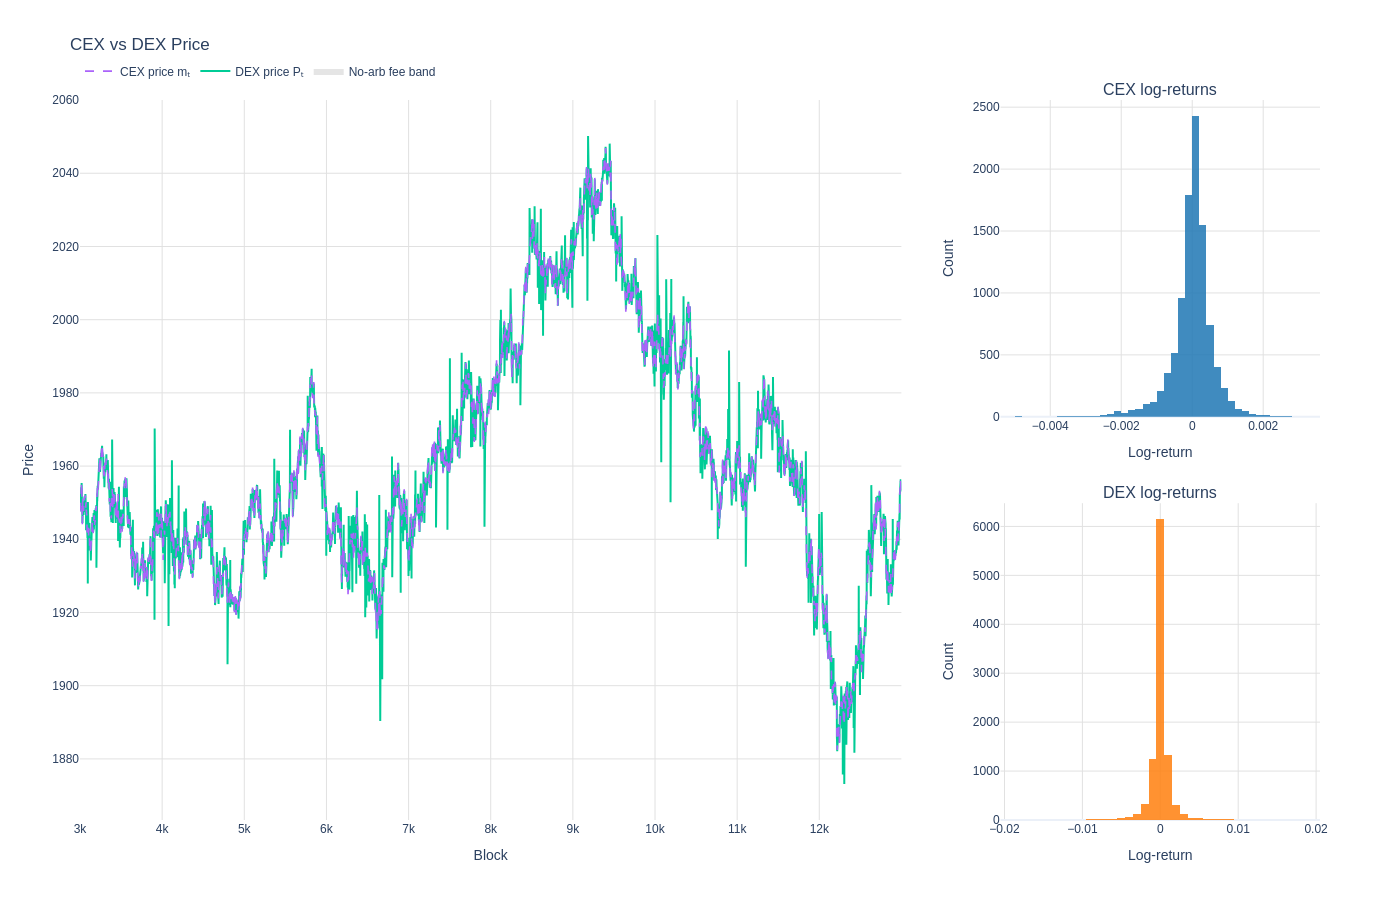
\includegraphics[width=0.7\linewidth]{images/259572_static_LPpassiveshare1_pjit0.0_1_price_steps10000.png}
    \caption{Evolution of DEX and CEX prices, together with the no arbitrage bands and the CEX and DEX log returns distributions. The CEX log returns distribution shows a negative skewness due to the negative correlation between price and volatility in the Heston dynamics. The remaining parameters are summarized in \ref{tab:common_params}.}
    \label{fig:cex_dex_prices}
\end{figure}

\begin{figure}
    \centering
    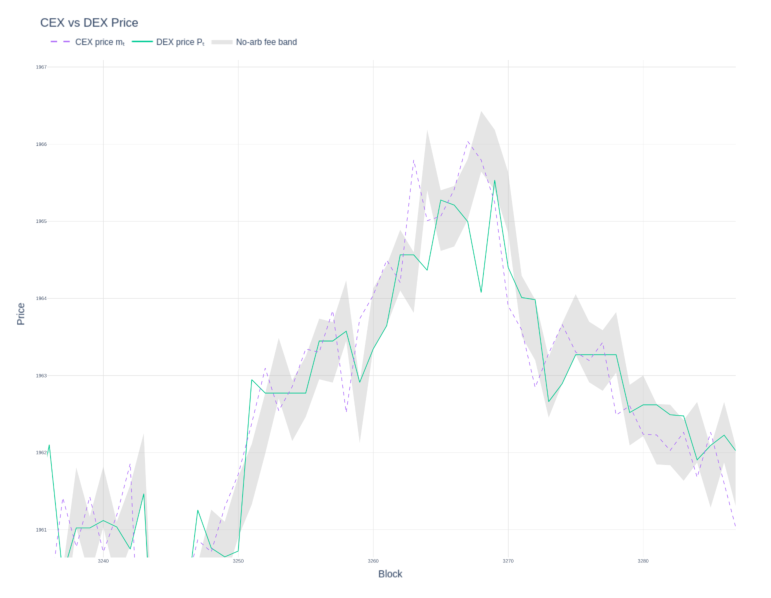
\includegraphics[width=0.6\linewidth]{images/cex_dex_band.pdf}
    \caption{Evolution of DEX and CEX prices, together with the no arbitrage bands zoomed in a small block intervals. The remaining parameters are summarized in \ref{tab:common_params}.}
    \label{fig:cex_dex_prices}
\end{figure}

Another interesting feature emerging from the ABM simulations under static fees (model 2) is the distinctive shape of the autocorrelation function (ACF) of end-of-block DEX prices. Figure \ref{fig:acf_dex} shows a pronounced negative spike at lag 1, indicating short-horizon mean reversion across consecutive blocks.

A qualitatively similar lag-1 anticorrelation has been documented in the empirical analysis of DEX prices by \cite{dinosse_gatta}, where it is associated with “reverse-trade” arbitrage dynamics as formalized in \cite{capponi2021liquidity}. In our setting, however, the mechanism is not driven by alternating trades within the DEX due to atomic arbitrage sequences. Rather, the effect arises from non-atomic CEX--DEX arbitrage executed at block granularity.

Our results suggest that block-time non-atomic arbitrage alone can produce the same qualitative lag-1 anticorrelation pattern observed empirically, providing an additional, and probably complementary, microstructural explanation for the lag-1 negative ACF documented in \cite{dinosse_gatta}.

\begin{figure}
    \centering
    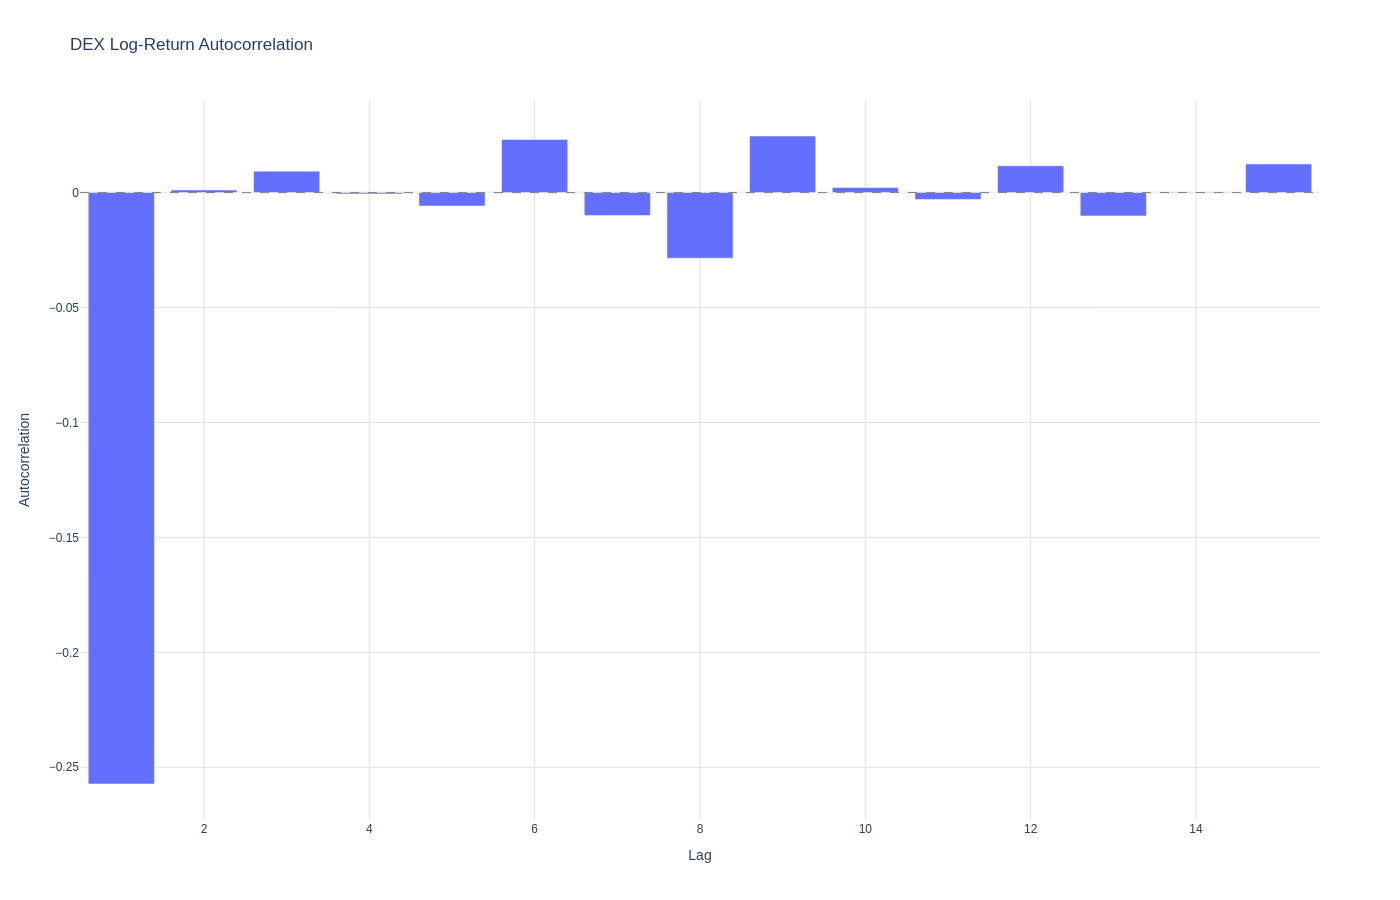
\includegraphics[width=0.5\linewidth]{images/274418_static_LPpassiveshare0.5_pjit0.0_1c_dex_return_acf_steps10000.png}
    \caption{Caption}
    \label{fig:acf_dex}
\end{figure}

\subsection{Baseline case}
We start from a fixed-fee environment, setting the liquidity-taker fee to its baseline value $f_t \equiv f_0 = 1\times 10^{-4}$ 
and keeping all remaining parameters as in Table \ref{tab:common_params}. :contentReference[oaicite:0]{index=0} Within each block, the reference (CEX) 
mid-price evolves while on-chain execution is deferred to the block boundary via a mempool replay; importantly, the arbitrage intent 
is executed first, so any profitable mispricing that survives fees and flash funding costs is harvested with priority.  Figure \ref{fig:cex_dex_prices} reports
the static-fee results for Model~0 (passive LPs only): the 
passive LP cohort exhibits persistently negative hedged PnL across the full horizon, while the arbitrageur realizes positive profits
and the noise trader loses, consistent with a microstructure channel in which block-time latency creates systematically stale AMM 
quotes that are picked off at the next block boundary. In this baseline configuration the 
smart router still finds the AMM competitive often enough that it routes about $35\%$ of trades to the DEX (Figure \ref{fig:trade_routing}), implying 
that the negative LP outcome is not driven by a collapse in order flow but by a structural wedge between fixed fee revenues and 
adverse-selection losses. Table \ref{tab:arb_detailed} further shows that arbitrage is frequent and stable 
already in Model~0 (about $9020$ executed arbitrage trades on average in the static-fee regime), reinforcing that LP underperformance 
is a persistent effect rather than a tail-event artifact. Model~1 adds an active LP cohort with 
narrower ranges, increasing depth locally around the prevailing price. In the static-fee case (Figure \ref{fig:lp_pnls}), 
both LP cohorts remain negative on a hedged basis, and the active cohort performs worse than the passive cohort, matching the expected 
concentration--LVR trade-off: concentrating liquidity can raise fee intensity when in-range, yet it magnifies the loss extracted by 
arbitrageurs when prices move across the local curve. In the static-fee case (Figure \ref{fig:lp_pnls}), 
both LP cohorts remain negative on a hedged basis, and the active cohort performs worse than the passive cohort, matching the expected 
concentration--LVR trade-off: concentrating liquidity can raise fee intensity when in-range, yet it magnifies the loss extracted by 
arbitrageurs when prices move across the local curve. The overall arbitrage intensity remains
comparable to Model~0 in the static regime (about $8696$ executed arbitrage trades on average), indicating that the deterioration
for active LPs is primarily a redistribution/amplification of LVR exposure rather than a qualitatively new arbitrage phase. 
Finally, Model~2 introduces a Just-in-Time (JIT) searcher (the Jiter), who temporarily 
supplies extremely narrow liquidity around the largest swap(s) and withdraws immediately after execution.  In the static-fee 
benchmark (Figure \ref{fig:lp_pnls}), the hedged PnLs of passive and active LPs remain negative with only marginal differences relative to Model~1,
while the Jiter ends up approximately break-even; the main reason is that successful JIT episodes are rare under a fixed low fee 
because fee income often fails to offset flash-loan financing costs.  In the same static setting, the DEX share remains non-trivial---
the median is reported around $43\%$---suggesting that, even with meaningful routed flow, a constant fee does not adapt to the 
time-varying intensity of stale-price risk created by block-time execution, leaving $F_t$ systematically dominated by 
$\mathrm{LVR}_t$ for longer-horizon LPs.  Taken together, the static-fee baseline establishes a clear ordering: the arbitrageur
earns persistently positive profits, the noise trader loses, and hedged LP profitability is structurally negative across increasing
model complexity; introducing active liquidity worsens hedged outcomes for the concentrated cohort, while introducing JIT liquidity does not
materially improve (and can potentially compete for) the fee stream available to longer-horizon LPs when fees are fixed. 



\subsection{Dynamic case}
\label{sec:dynamic_fees}

We now replace the constant taker fee with an adaptive fee process following the rules in Section~\ref{subsec:fees}, and 
we study three schedules: a toxicity-driven mechanism (fees increase when order flow is more adverse-selection-intensive) 
and two volatility-driven mechanisms based on realized volatility (computed either from DEX prices or from the CEX reference). 
Relative to the static benchmark, the core economic role of dynamic fees is to endogenously widen the no-arbitrage band in 
precisely those periods in which stale-quote risk is high, thereby reducing the fraction of blocks in which priority arbitrage 
can profitably pick off the pool and transferring a larger share of surplus to liquidity providers through higher fee revenues. 
This trade-off is visible already in Model~0 (arbitrageur + noise trader + smart router + passive LPs): under toxicity-driven fees, 
the passive LP’s hedged PnL becomes persistently positive over the full horizon and, on average, exceeds the arbitrageur’s profits
 (Figure~\ref{fig:model0_pnls_toxicity}), while the noise trader remains structurally negative and the smart router stays close to 
 break-even as expected in a competitive routing environment. The corresponding empirical fee distribution and routed market share 
 remain in plausible ranges (Figure~\ref{fig:model0_fee_toxicity}): the upper quartile of fees is around $0.1\%$, with occasional 
 realizations above $1\%$, and the DEX market share decreases relative to the static case but stabilizes around $25\%$, indicating 
 that adaptivity can restore LP profitability without collapsing activity on the pool. A similar, though quantitatively milder, 
 improvement is obtained with volatility-based fees: when fees are driven by DEX volatility, the passive LP remains consistently 
 profitable but earns less than under toxicity-driven fees, while operating at lower fee levels throughout the simulation (
  Figure~\ref{fig:model0_pnls_voldex} and Figure~\ref{fig:model0_fee_voldex}); volatility computed from the CEX reference delivers 
  results of the same qualitative type. The arbitrage diagnostics in Table~\ref{tab:arb_detailed} corroborate the mechanism: across 
  all dynamic schedules, executed arbitrage trades drop markedly in Model~0 (from about $9020$ in the static case to roughly $5843$ 
  under toxicity and $5892$--$6360$ under volatility-based rules), while ``No Arb'' cases rise correspondingly, consistent with a 
  widened fee-implied band that makes fewer price discrepancies profitable to exploit.

Introducing active LPs (Model~1) changes the distribution of fee revenues and adverse-selection exposure, but the same basic logic 
applies: dynamic fees improve LP outcomes relative to the static benchmark, yet the benefit depends sharply on how well the fee rule 
targets toxicity rather than generic volatility. In particular, the toxicity-driven schedule is the only configuration under which 
both passive and active LPs achieve positive hedged profits, whereas volatility-based schedules push the passive LP close to break-even 
while the active LP remains negative on a hedged basis (Figure~\ref{fig:model1_pnls_toxicity} and Figure~\ref{fig:model1_fee_volcex}). 
This asymmetry is economically coherent with concentrated liquidity: active LPs earn higher fee intensity when in-range, but they also 
bear amplified LVR for a given amount of price movement, so a volatility proxy that does not sufficiently discriminate toxic flow from 
benign flow tends to under-compensate active ranges exactly when arbitrage selection is most severe; conversely, toxicity-driven fees 
increase precisely during adverse selection episodes and can offset the higher LVR exposure induced by concentration. 
Table~\ref{tab:arb_detailed} again supports the interpretation: relative to static, arbitrage execution falls under all dynamic 
schedules (e.g., from about $8696$ to about $5529$ in the toxicity case), suggesting that improved LP outcomes are primarily associated 
with fee adaptivity reducing the exploitable stale-quote component rather than with a change in the underlying price process.

Finally, Model~2 adds the JIT liquidity searcher (the Jiter), and this introduces a qualitatively different interaction: 
fee adaptivity can make JIT fee-capture profitable, but that same profitability can come at the expense of longer-horizon LPs 
because JIT liquidity is deployed exactly around the largest swaps, i.e., where most fee mass is generated. In the dynamic-fee 
regimes, the Jiter becomes profitable (Figures~\ref{fig:pnl_model2_toxicity} and \ref{fig:pnl_model2_volcex}), reflecting a reduced 
LVR-to-fee ratio over the JIT holding window and a higher fee level in the very blocks in which JIT deploys; however, across all
 tested dynamic schedules, neither passive nor active LPs achieve consistent positive hedged profits in the presence of JIT liquidity. 
 This outcome is economically plausible in our setting: dynamic fees increase the fee pool available precisely in the blocks that 
 trigger JIT entry, and the Jiter captures a dominant fraction of that fee flow by construction, mechanically reducing the fees 
 accruing to other LPs while leaving their exposure to block-time adverse selection only partially mitigated. Consistent with the 
 earlier models, arbitrage-related counts remain broadly stable across specifications (Table~\ref{tab:arb_detailed}), so the 
 deterioration for non-JIT LPs in Model~2 is best understood as a redistribution of fee income toward the Jiter rather than as a 
 resurgence of arbitrage intensity. Taken together, these results show that adaptive fees can robustly restore LP profitability in 
 the absence of JIT liquidity (Model~0) and can even support both passive and active LP profitability when fees are tied directly 
 to toxicity (Model~1), but that, once JIT fee-sniping is admitted (Model~2), fee adaptivity alone is insufficient to protect 
 longer-horizon LPs because the mechanism that stabilizes LP returns also increases the value of JIT entry in the highest-fee blocks.


% \subsection{Model 0}
% In this initial version, we let only the arbitrageur, the noise trader and the passive LP to act. We want to answer the following questions:
% \begin{enumerate}
%     \item In the static fee case, how does the hedged passive LP PnL behave?
%     % \item Keeping the fee fixed, how does hedged passive LP PnL change according to LP activities?
%     \item If we allow the fee to change, what changes with respect to the static case? 
%     \item Are we able to keep DEX attractive and have positive hedged LP PnLs?
% \end{enumerate}

% To answer the first question, we can look at Figure \ref{fig:model0_pnls_0}. It shows the agents' PnLs across 50 runs of the simulation via the mean and plus/minus two standard deviations. In a static fee case, the hedged passive LP PnL is always smaller that zero.

\begin{figure}
    \centering
    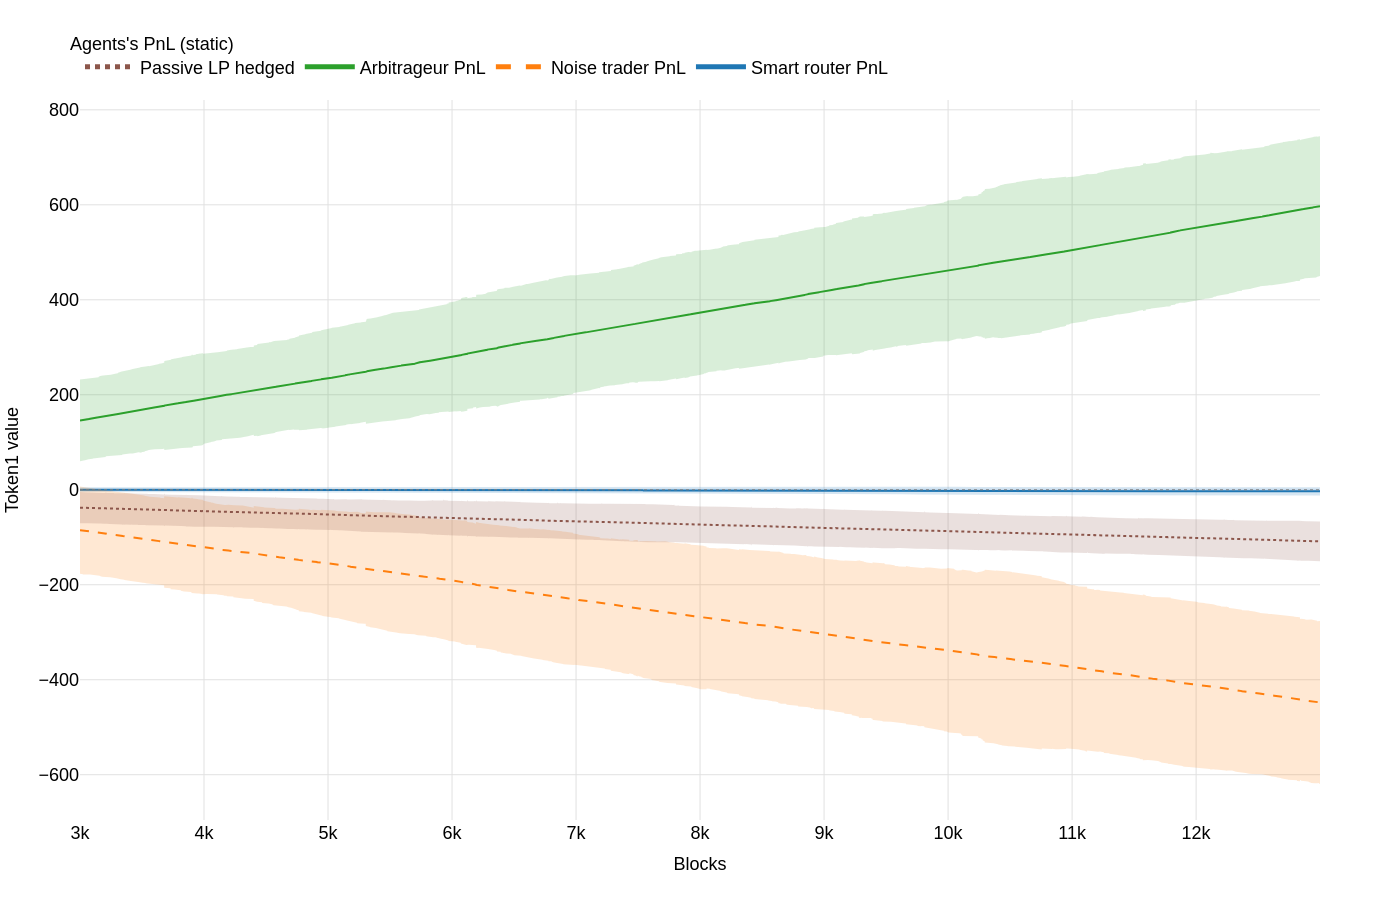
\includegraphics[width=0.8\linewidth]{images/pnl_static_test_runs50_LPpassiveshare1_pjit0_293410.png}
    \caption{Agents' PnLs averaged across 50 runs in the static fee case for model 0. The dashed area around the mean corresponds to plus/minus two standard deviations. The remaining parameters are summarized in \ref{tab:common_params}.}
    \label{fig:model0_pnls_0}
\end{figure}

% As shown in Figure \ref{fig:model0_fee_dexshare_0}, the smart router routes approximately 35\% of trades to the AMM rather than the CEX. This value appears reasonable in the present setting. In practice, order-routing decisions may reflect considerations beyond immediate price optimality, such as participation in broader strategies involving multiple pools or DEXs. From this perspective, a DEX share of 35\% can be interpreted as a conservative, or pessimistic, outcome.

\begin{figure}
    \centering
    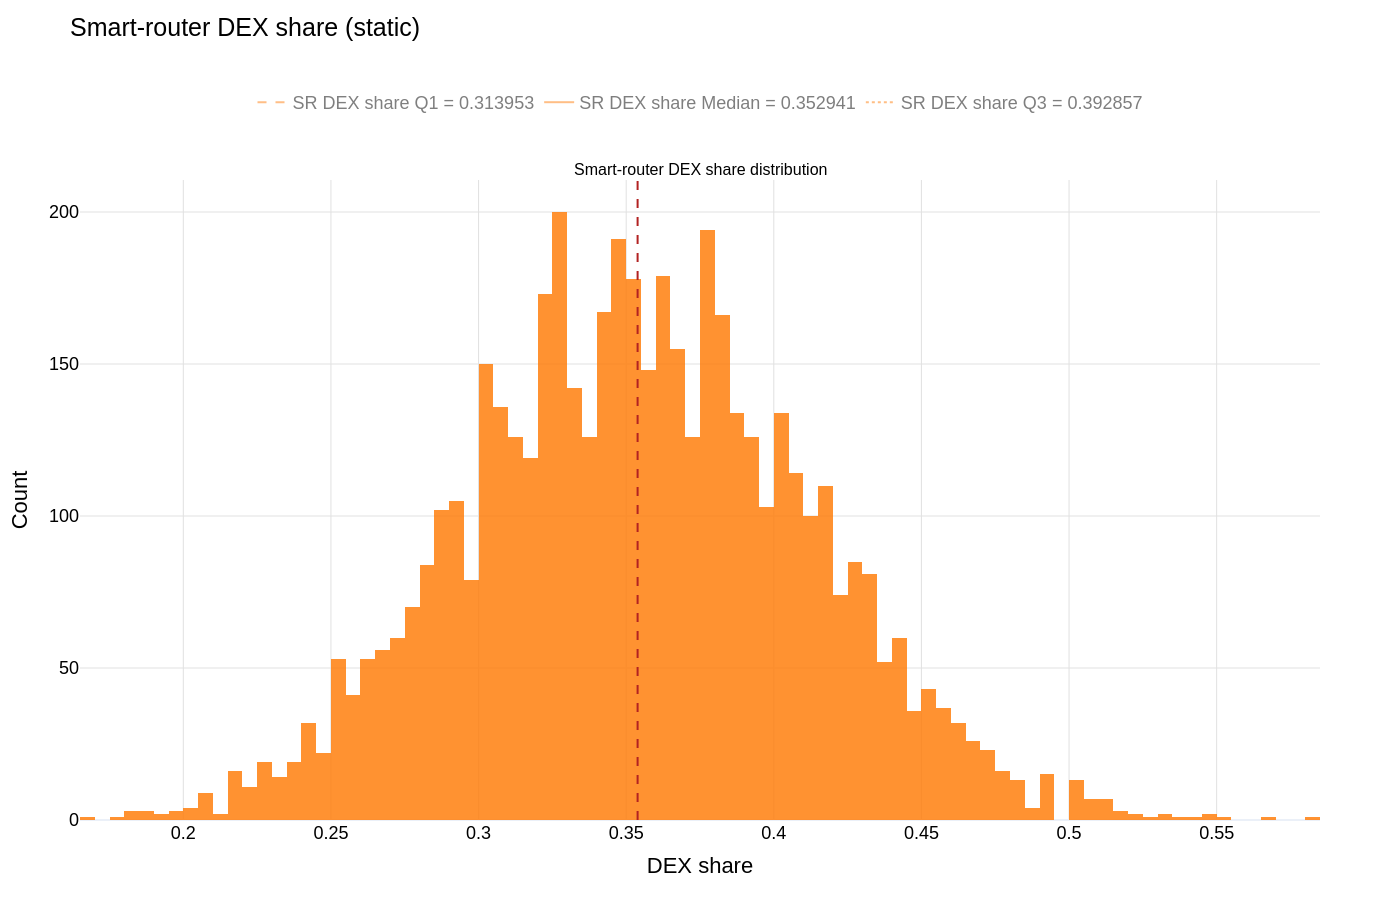
\includegraphics[width=0.5\linewidth]{images/fee_static_model0_runs50_LPpassiveshare1_pjit0_271886.png}
    \caption{Static fee and DEX share empirical distribution across 50 runs for model 0. The remaining parameters are summarized in \ref{tab:common_params}.}
    \label{fig:model0_fee_dexshare_0}
\end{figure}

% We now allow the trading fee to vary according to the rules described in Section \ref{subsec:fees}. Among all the fee schedules considered, the toxicity-driven fee dynamics yields the most favorable outcome from the liquidity providers’ perspective, as shown in Figure \ref{fig:model0_pnls_toxicity}. The hedged passive PnL remains positive over the entire simulation horizon and exceeds the arbitrageur’s profits. As expected, noise traders incur negative PnLs, while smart routers exhibit PnLs close to zero.

% The corresponding fee levels and DEX market share, reported in Figure \ref{fig:model0_fee_toxicity}, remain within reasonable ranges. In particular, the third quartile of the fee is approximately $0.1\%$, although occasional realizations exceed $1\%$.

\begin{figure}
    \centering
    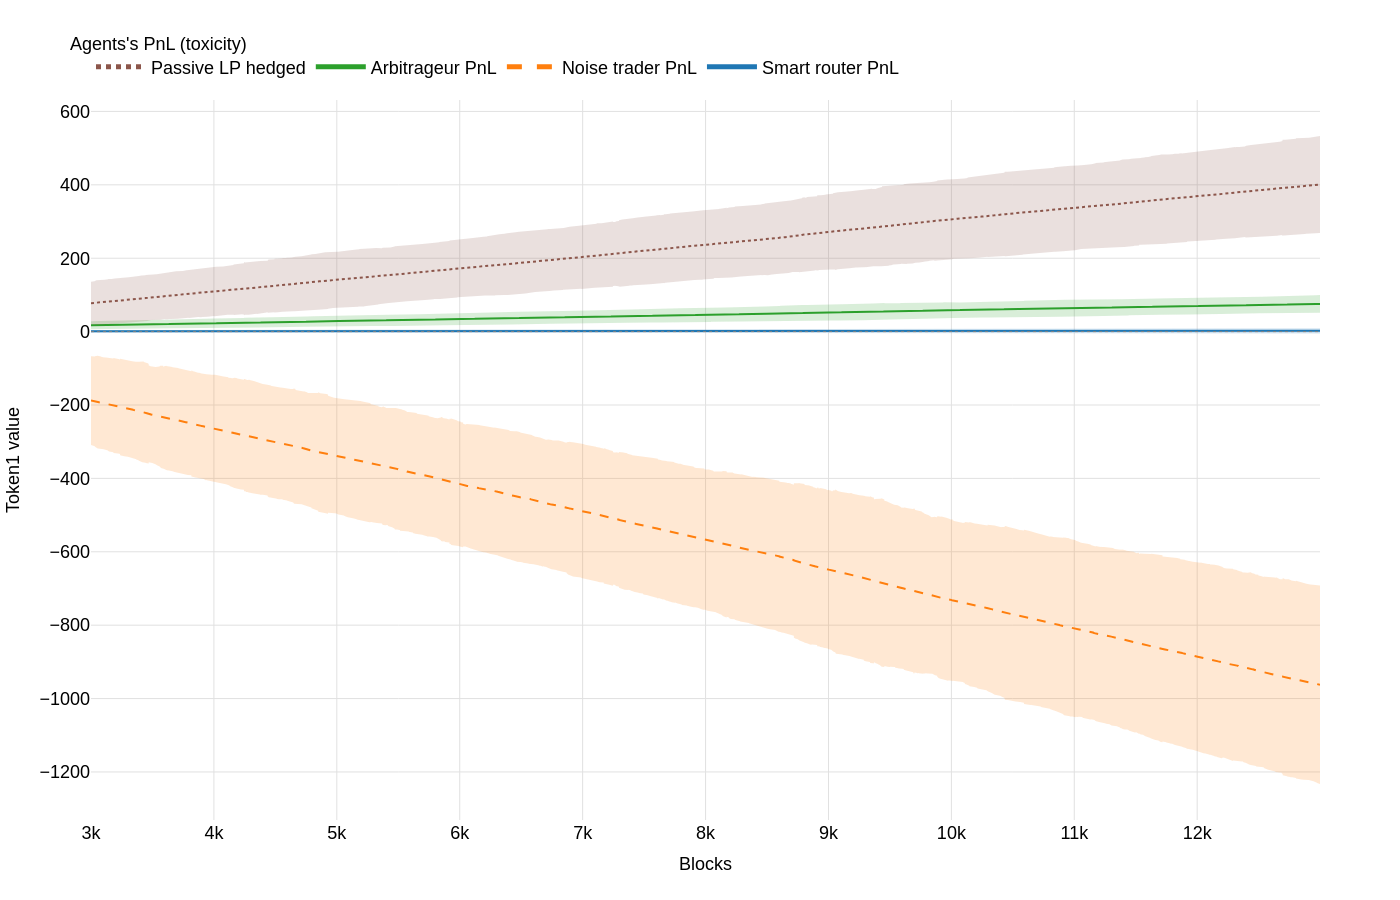
\includegraphics[width=0.8\linewidth]{images/pnl_toxicity_test_runs50_LPpassiveshare1_pjit0_293410.png}
    \caption{Agents' PnLs averaged across 50 runs in the toxicity-driven fee case for model 0. The dashed area around the mean corresponds to plus/minus two standard deviations. The remaining parameters are summarized in \ref{tab:common_params}.}
    \label{fig:model0_pnls_toxicity}
\end{figure}


\begin{figure}
    \centering
    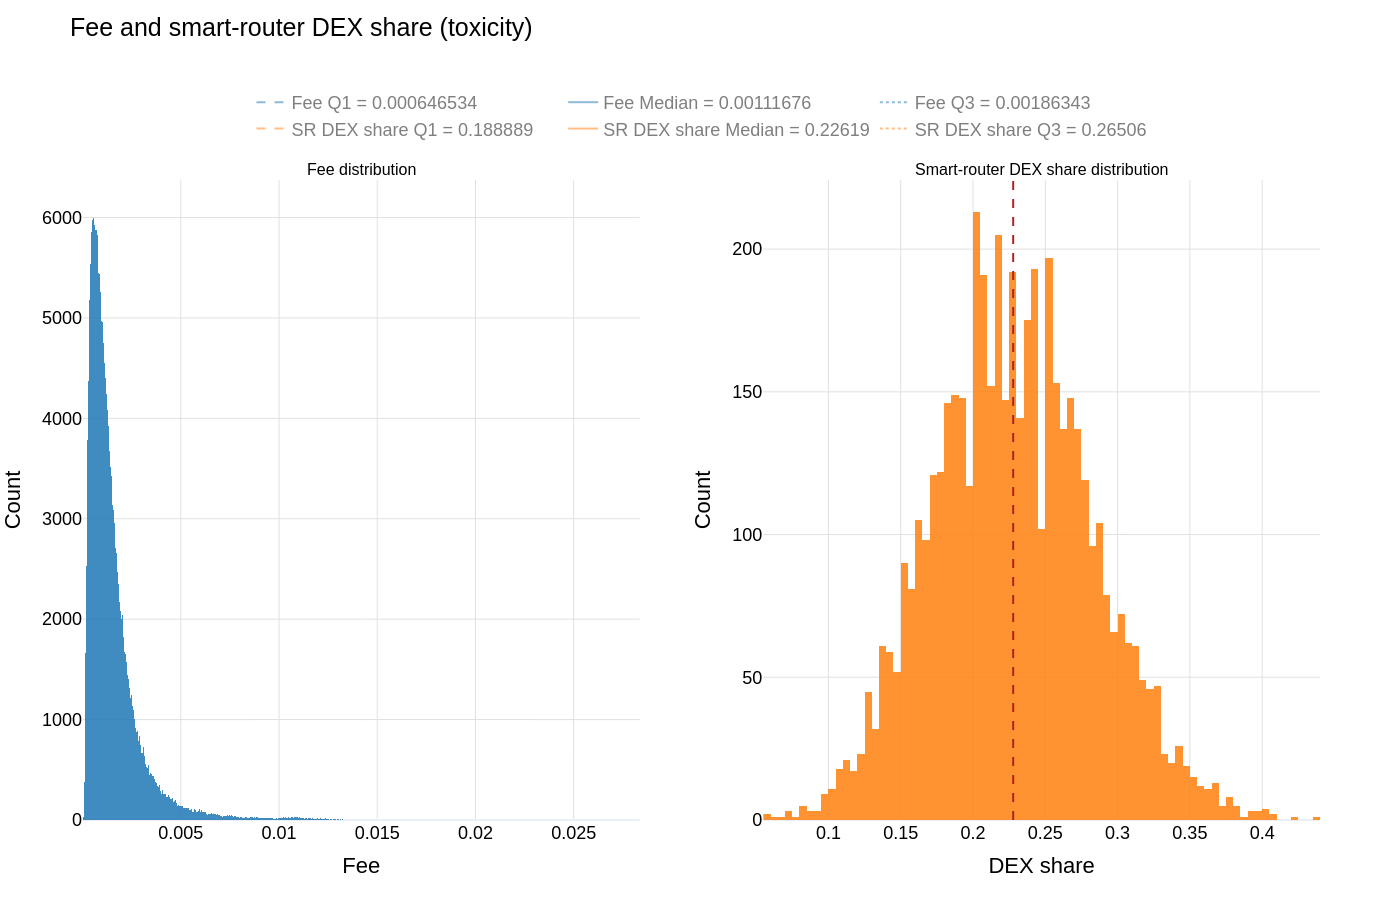
\includegraphics[width=0.8\linewidth]{images/fee_toxicity_test_runs50_LPpassiveshare1_pjit0_293410.png}
    \caption{Toxicity-driven fee and DEX share empirical distribution across 50 runs for model 0. The remaining parameters are summarized in \ref{tab:common_params}.}
    \label{fig:model0_fee_toxicity}
\end{figure}

% As expected, the DEX market share decreases relative to the static-fee benchmark; nevertheless, it remains stable at approximately 25\%.

% We also obtain robust results when fees are determined by DEX-specific volatility. In this setting, the model consistently maintains positive LP profits, although these profits are lower than those observed under the toxicity-based fee mechanism. Importantly, this is achieved while sustaining lower fee rates throughout the entire simulation horizon. The corresponding results are reported in Figures \ref{fig:model0_pnls_voldex} and \ref{fig:model0_fee_voldex}.

\begin{figure}
    \centering
    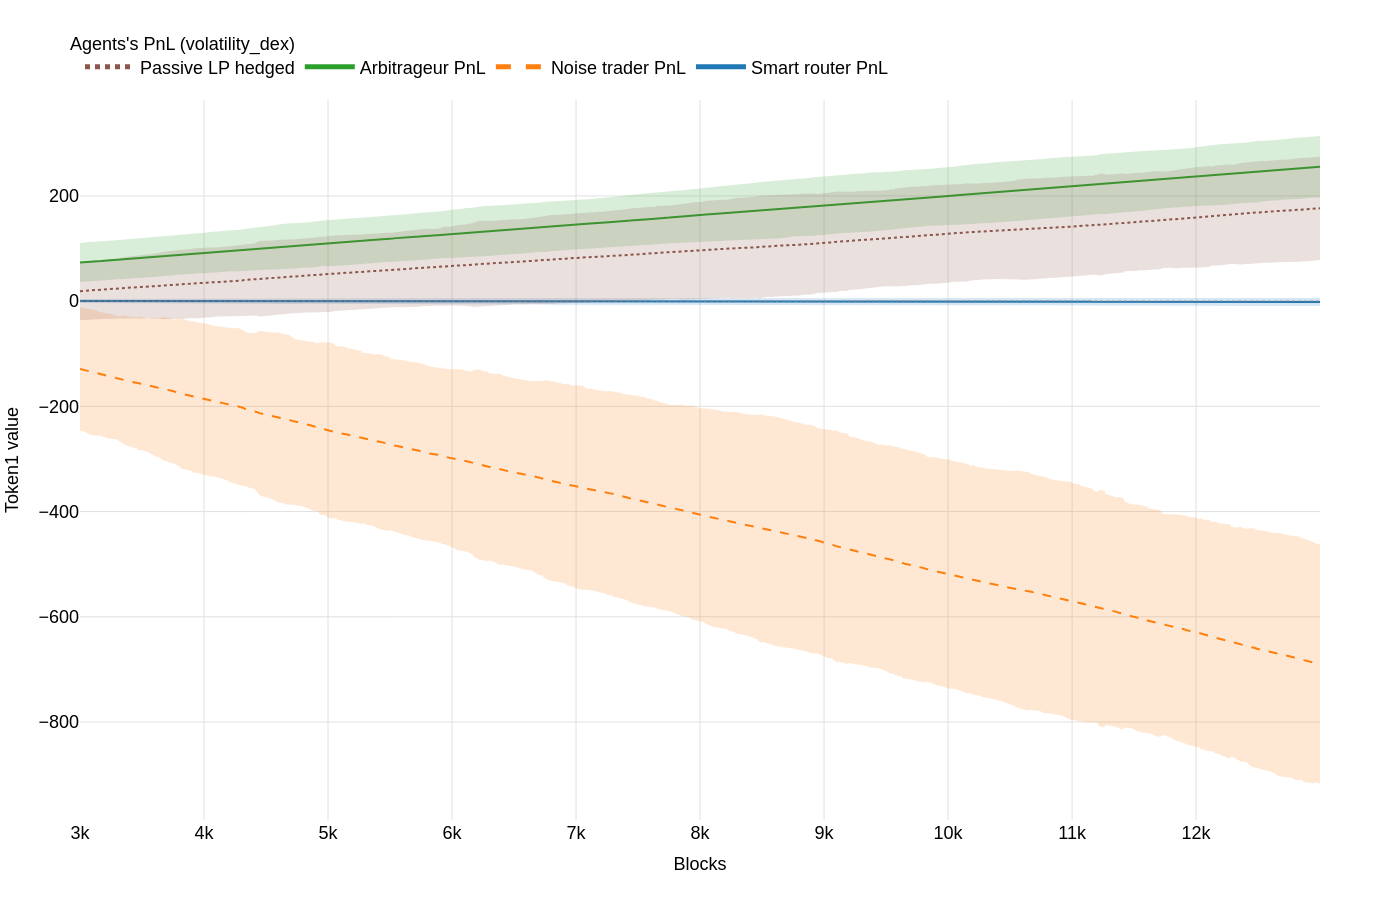
\includegraphics[width=0.8\linewidth]{images/pnl_volatility_dex_test_runs50_LPpassiveshare1_pjit0_293410.png}
    \caption{Agents' PnLs averaged across 50 runs in the DEX volatility-driven fee case for model 0. The dashed area around the mean corresponds to plus/minus two standard deviations. The remaining parameters are summarized in \ref{tab:common_params}.}
    \label{fig:model0_pnls_voldex}
\end{figure}


\begin{figure}
    \centering
    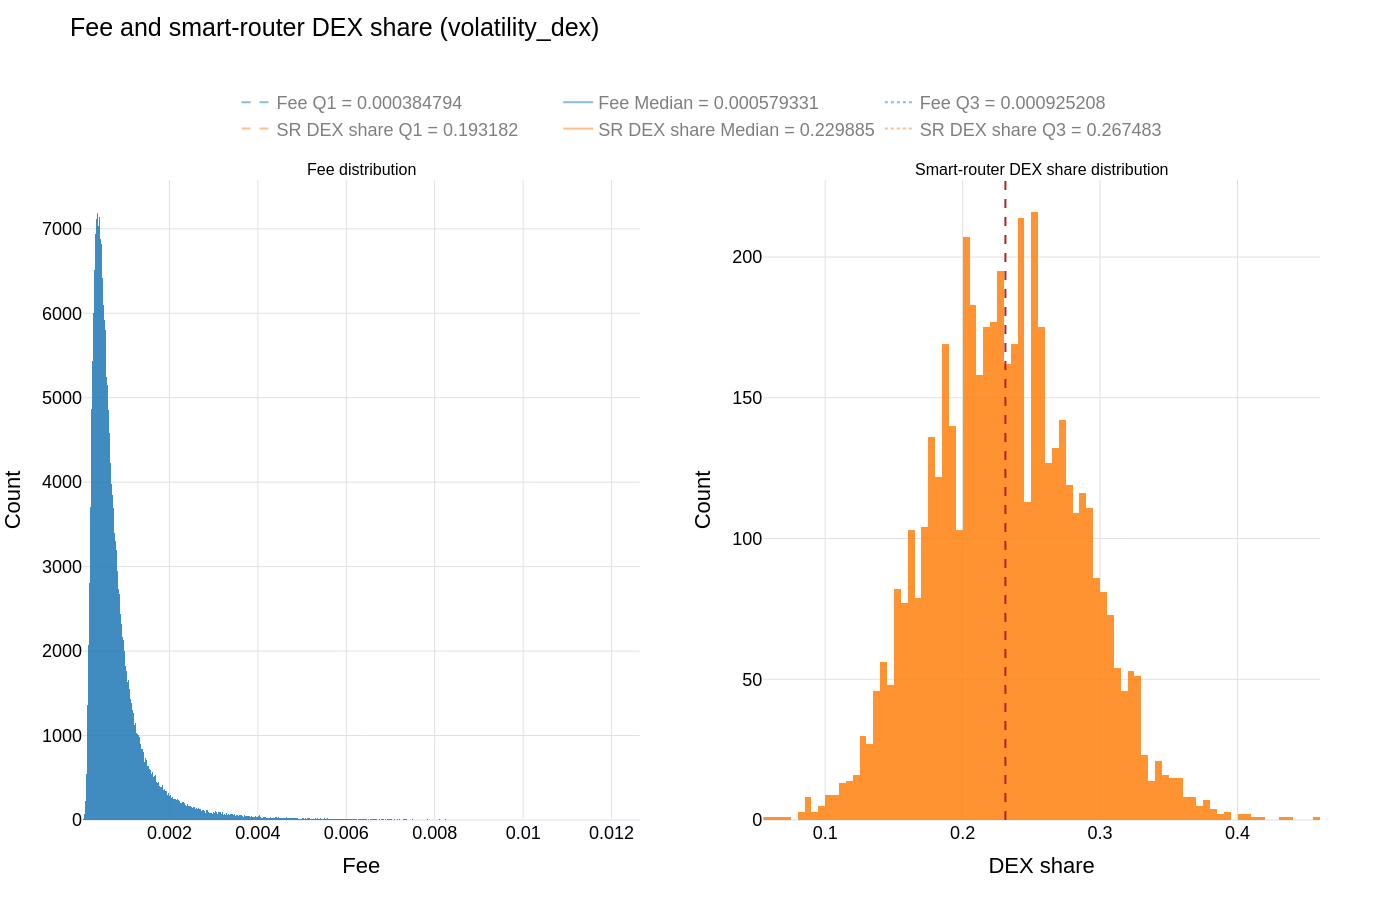
\includegraphics[width=0.8\linewidth]{images/fee_volatility_dex_test_runs50_LPpassiveshare1_pjit0_293410.png}
    \caption{DEX volatility-driven fee and DEX share empirical distribution across 50 runs for model 0. The remaining parameters are summarized in \ref{tab:common_params}.}
    \label{fig:model0_fee_voldex}
\end{figure}



% \subsection{Model 1}
% As previously discussed, Model 1 introduces active LPs as a fraction of the total LP population \(N_{\text{LP}}\). 
% As expected, increasing the number of active LPs primarily redistributes profits away from passive LPs. For this reason, 
% in the following analysis we fix the population to \(N_{\text{LP}}/2\) active LPs and \(N_{\text{LP}}/2\) passive LPs.

% Figure \ref{fig:model1_pnls_static} reports the PnLs of all agents included in this model specification. As in previous settings, the arbitrageur realizes positive profits, the noise trader incurs losses, the smart router remains approximately break-even, and the passive LP exhibits negative PnL. The newly introduced active LP performs even worse in terms of hedged PnL relative to the passive LP. This outcome is attributable to the narrower liquidity ranges, which amplify LVR, as discussed in \cite{milionis2023}.

\begin{figure}
    \centering
    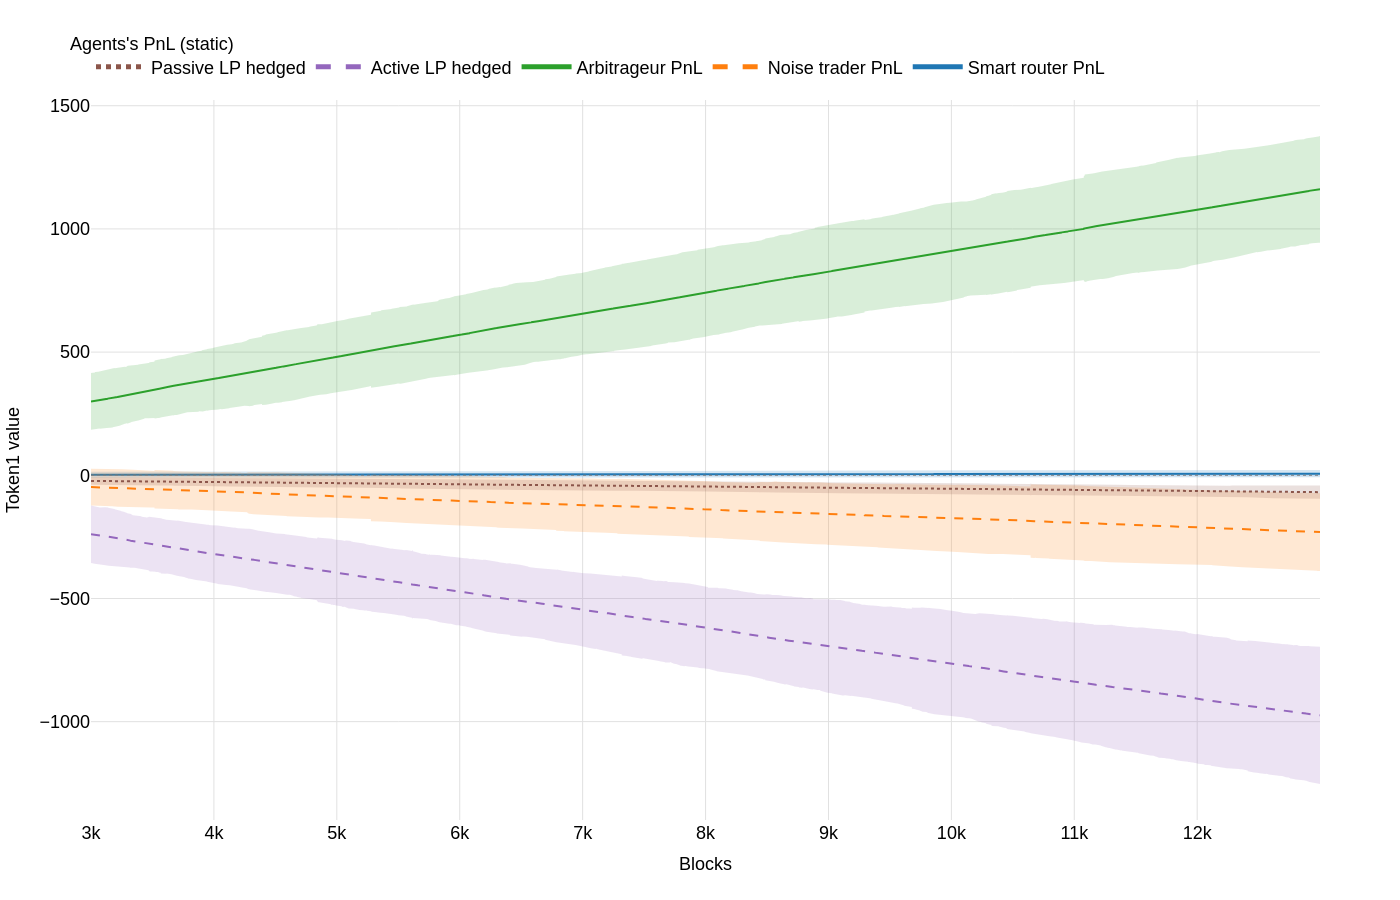
\includegraphics[width=0.8\linewidth]{images/pnl_static_test_runs50_LPpassiveshare0.5_pjit0_296795.png}
    \caption{Agents' PnLs averaged across 50 runs in the static fee case for model 1. The dashed area around the mean corresponds to plus/minus two standard deviations. The remaining parameters are summarized in \ref{tab:common_params}.}
    \label{fig:model1_pnls_static}
\end{figure}

% The introduction of active LPs leads to a substantial increase in the DEX market share, as shown in Figure \ref{fig:model1_fee_static}. This effect is likely driven by the higher concentration of liquidity around the prevailing DEX price, which enables the arbitrageur to execute profitable trades more frequently. Consistently, the arbitrageur’s PnL is higher in this setting than in Model 0. Enhanced arbitrage activity improves the alignment between DEX and CEX prices, thereby increasing the likelihood that the DEX offers a more competitive quote than the CEX.

\begin{figure}
    \centering
    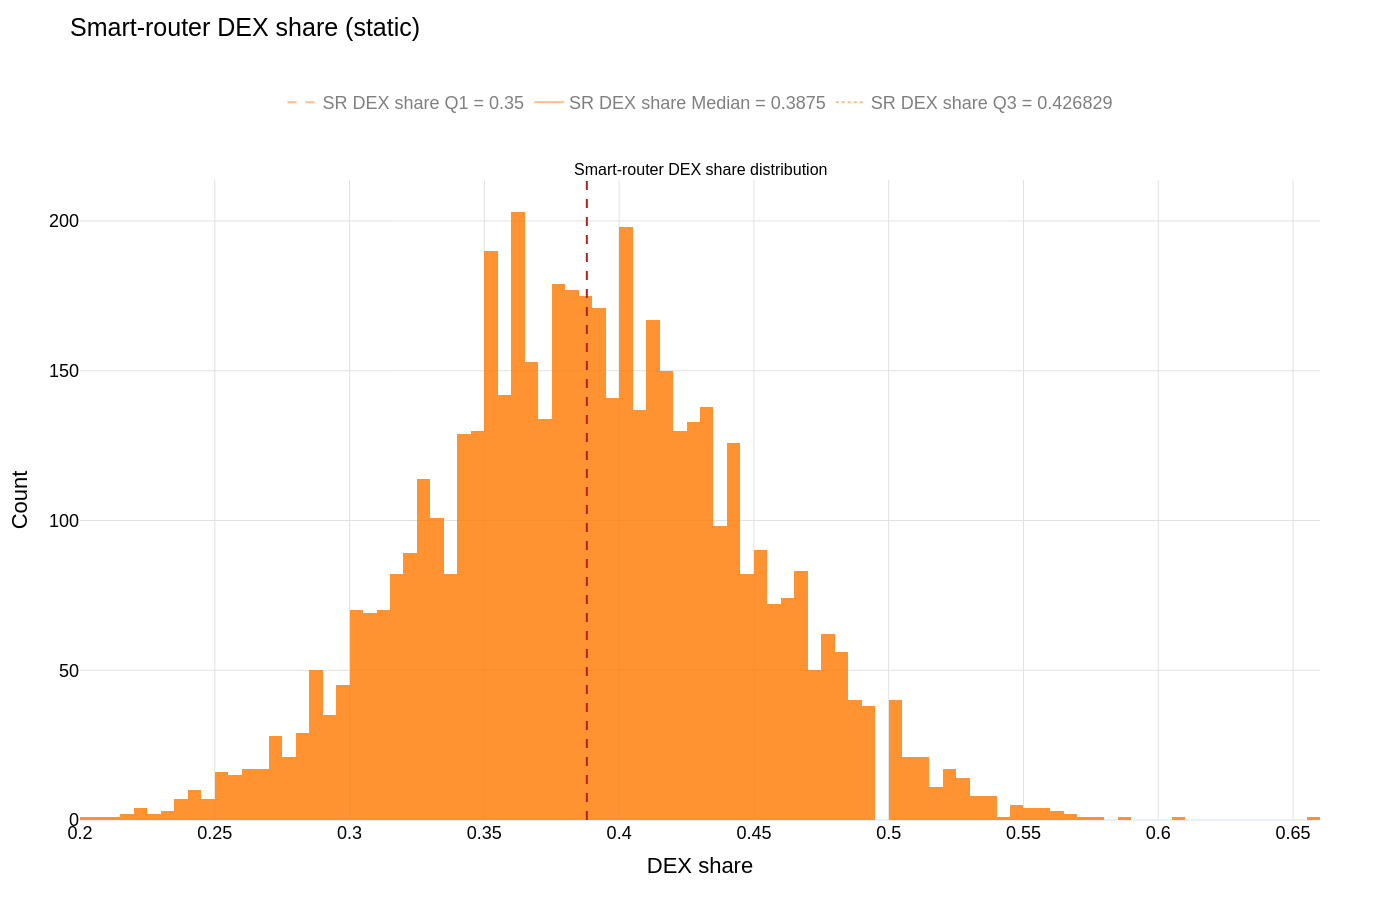
\includegraphics[width=0.5\linewidth]{images/fee_static_model1_runs50_LPpassiveshare0.5_pjit0_272506.png}
    \caption{DEX volatility-driven fee and DEX share empirical distribution across 50 runs for model 1. The remaining parameters are summarized in \ref{tab:common_params}.}
    \label{fig:model1_fee_static}
\end{figure}

% Also in this setting, the toxicity-driven fee schedule emerges as the most favorable from the liquidity providers’ perspective. It is, in fact, the only specification under which both active and passive LPs achieve positive hedged profits. Volatility-based fee schedules yield hedged PnL close to zero for passive LPs, but active LPs continue to experience negative hedged returns. These results are illustrated in Figures \ref{fig:model1_pnls_toxicity} and \ref{fig:model1_fee_volcex}.


\begin{figure}
    \centering
    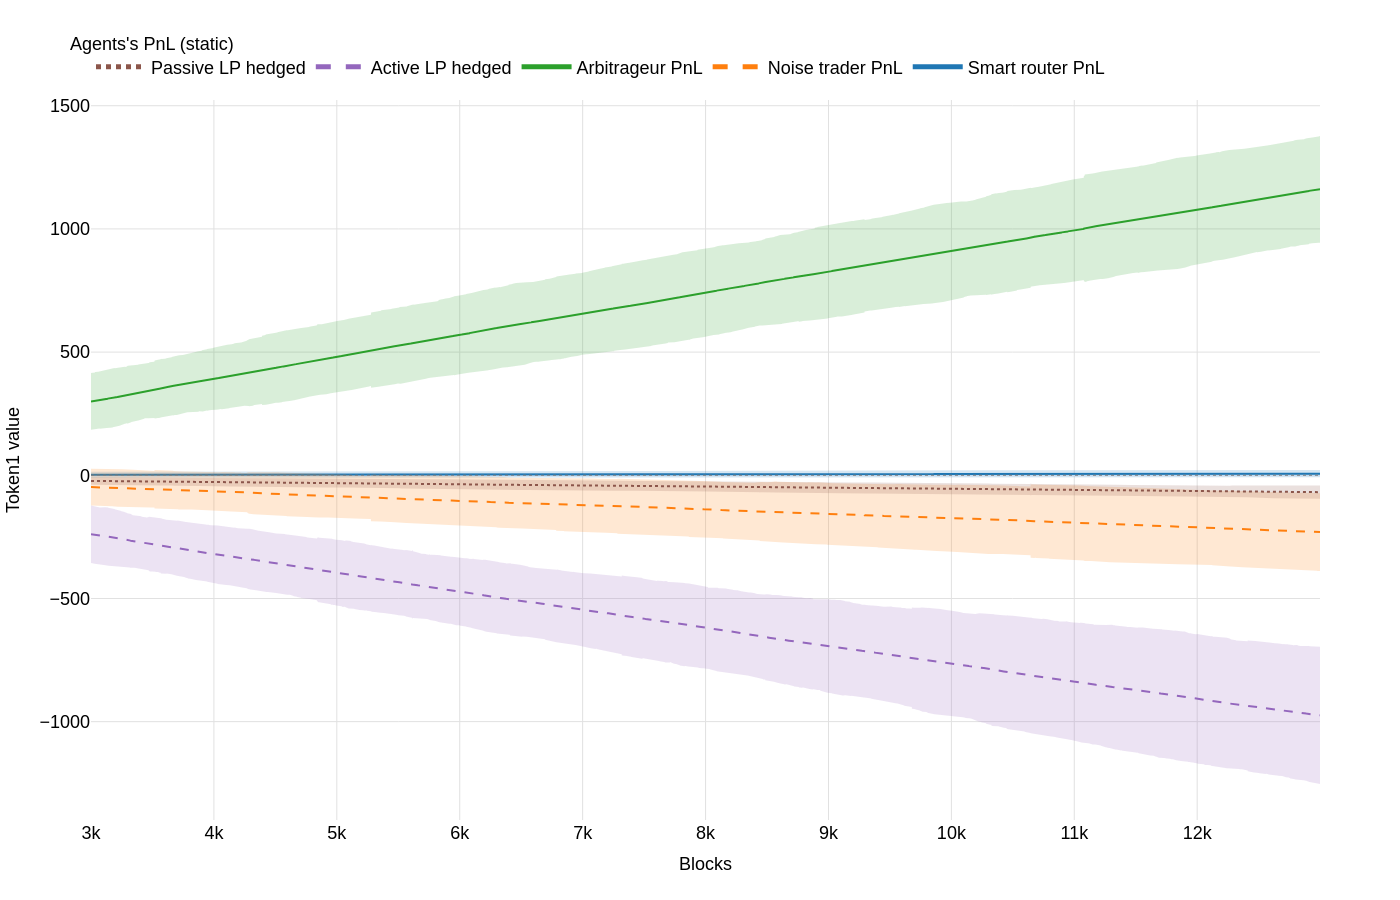
\includegraphics[width=0.5\linewidth]{images/pnl_static_test_runs50_LPpassiveshare0.5_pjit0_296795.png}
    \caption{Agents' PnLs averaged across 50 runs in the toxicity fee case for model 1. The dashed area around the mean corresponds to plus/minus two standard deviations. The remaining parameters are summarized in \ref{tab:common_params}.}
    \label{fig:model1_pnls_toxicity}
\end{figure}

\begin{figure}
    \centering
    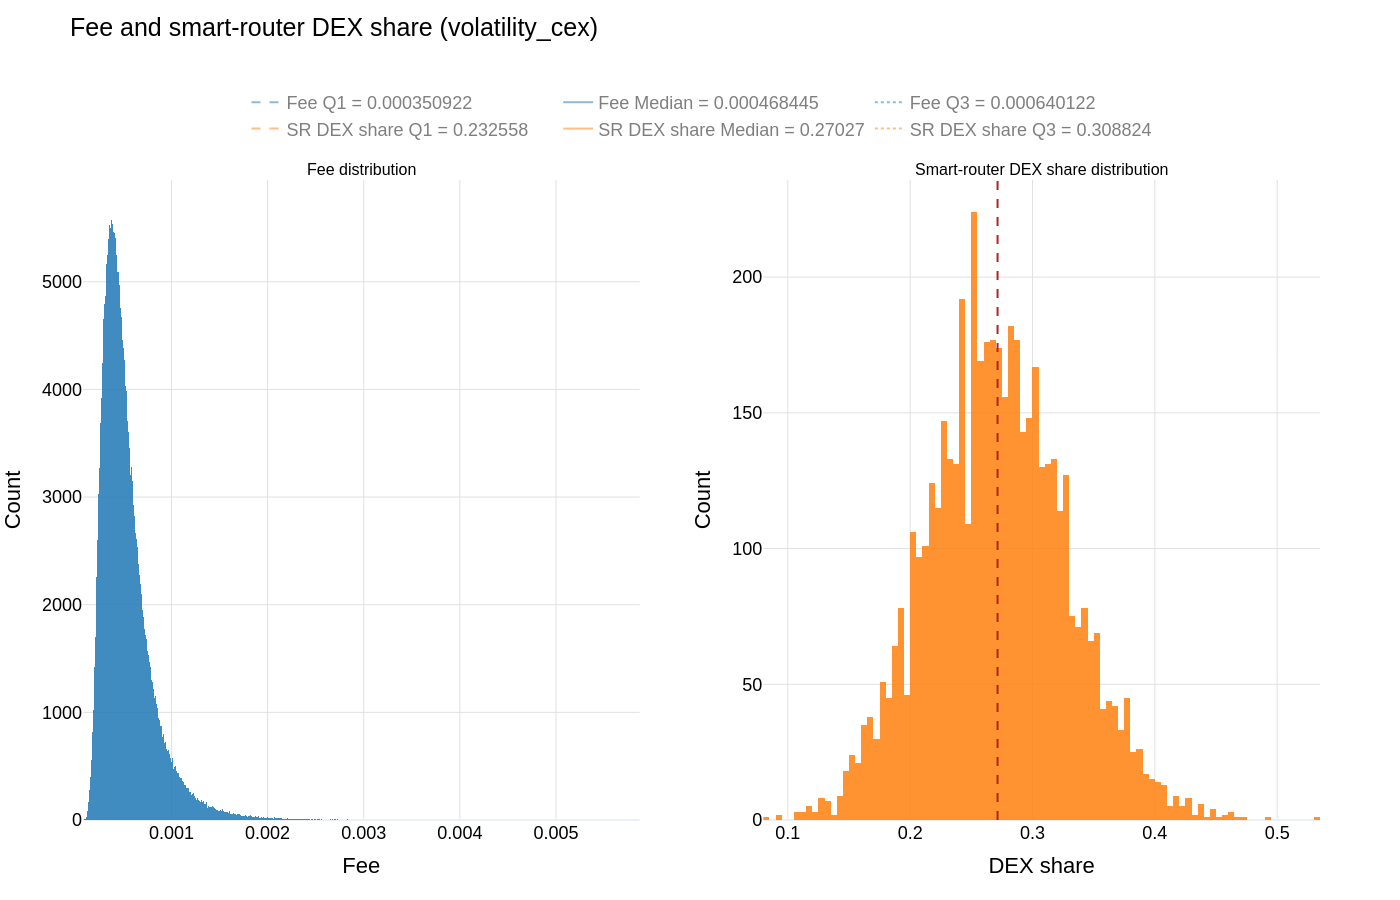
\includegraphics[width=0.8\linewidth]{images/fee_volatility_cex_test_runs50_LPpassiveshare0.5_pjit0_296795.png}
    \caption{CEX volatility-driven fee and DEX share empirical distribution across 50 runs for model 1. The remaining parameters are summarized in \ref{tab:common_params}.}
    \label{fig:model1_fee_volcex}
\end{figure}

% \subsection{Model 2}
% We conclude by introducing the final agent considered in our framework: the MEV searcher implementing a Just-in-Time (JIT) liquidity provision strategy, the Jiter. A JIT strategy is a specialized form of active liquidity provision in which the searcher supplies liquidity over an extremely narrow price range immediately before a swap and withdraws this liquidity and the accrued fees immediately after the swap is executed. This approach enables the searcher to capture nearly the entire fee paid by the liquidity taker while keeping exposure to LVR minimal, as the position is held only for a few micro-steps. Although the narrow range increases LVR on a per-step basis, the overall exposure remains limited due to the very short holding period.

% In the static case, the results regarding the hedged PnLs of liquidity providers (LPs) show only marginal differences across the various model specifications. As illustrated in Figure \ref{fig:pnl_model2_static}, both passive and active LPs experience negative hedged profits. Additionally, the Jiter position ends up nearly breaking even. This is mainly due to the very few cases of successful JIT caused by where the fee revenue offsets the flash loan costs. Also the DEX share median is similar to the other static cases, with a value of approximately 43\%. 

% \begin{figure}[h]
%   \centering
%   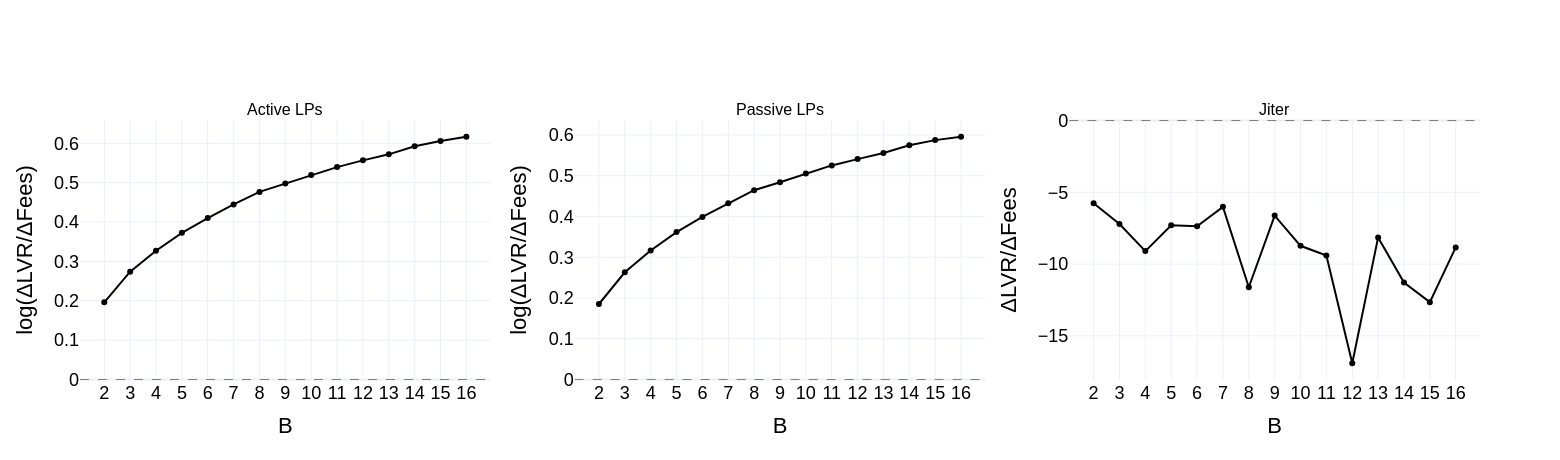
\includegraphics[width=\linewidth]{images/dLVR_over_dFees_medians_vs_block_time_static_flow_test_runs50_pid42657.png}
%   \caption{Static fees, active+passive LPs and Jiter: median and 95\% interval of $r=\Delta\mathrm{LVR}/\Delta\mathrm{Fees}$ vs $B$.}
%   \label{fig:static_with_jiter_ratio}
% \end{figure}

\begin{figure}
    \centering
    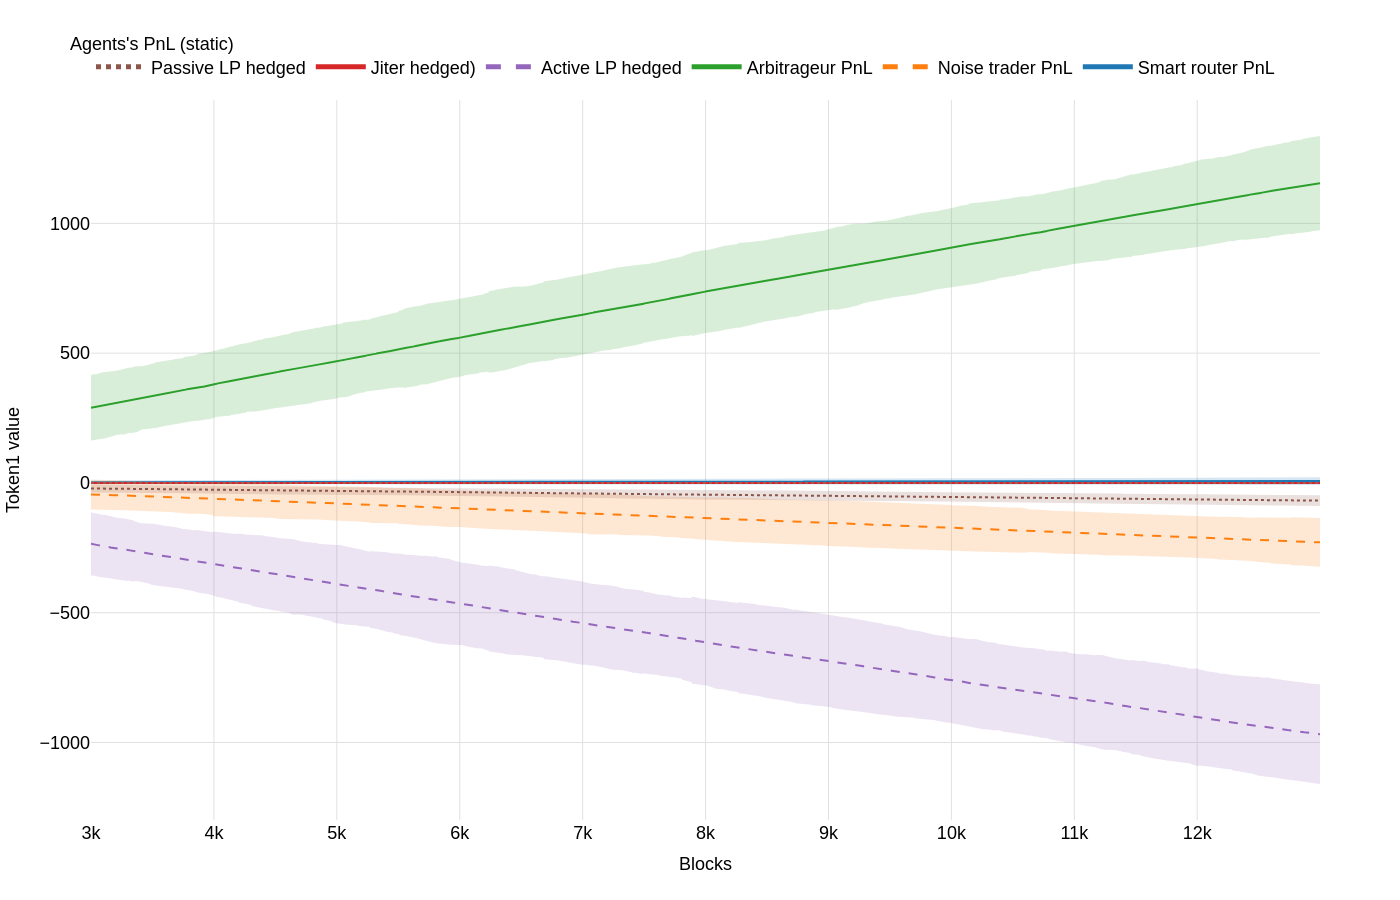
\includegraphics[width=0.8\linewidth]{images/pnl_static_test_runs50_LPpassiveshare0.5_pjit1_141947.png}
    \caption{Agents' PnLs averaged across 50 runs in the static fee case for model 2. The dashed area around the mean corresponds to plus/minus two standard deviations. The remaining parameters are summarized in \ref{tab:common_params}.}
    \label{fig:pnl_model2_static}
\end{figure}

% The introduction of dynamic fee rates significantly alters the economic outcome for the Jiter, resulting in a profit, but leads to a loss for the other LPs. The reduction in LVR relative to the fees helps push the Jiter's hedged PnL into positive territory. However, no dynamic fee schedule was able to generate consistent positive profits for both passive and active LPs. This outcome is reasonable, as the Jiter captures nearly all of the share in the price range where the largest swaps per block occur, thereby significantly reducing the fees earned by the other LPs. For further details, see Figures \ref{fig:pnl_model2_toxicity} and \ref{fig:pnl_model2_volcex}, where the results obtained with DEX volatility-driven fees are similar to those in the CEX volatility-driven case. There are no significant changes in the fee and DEX share distributions.



\begin{figure}
    \centering
    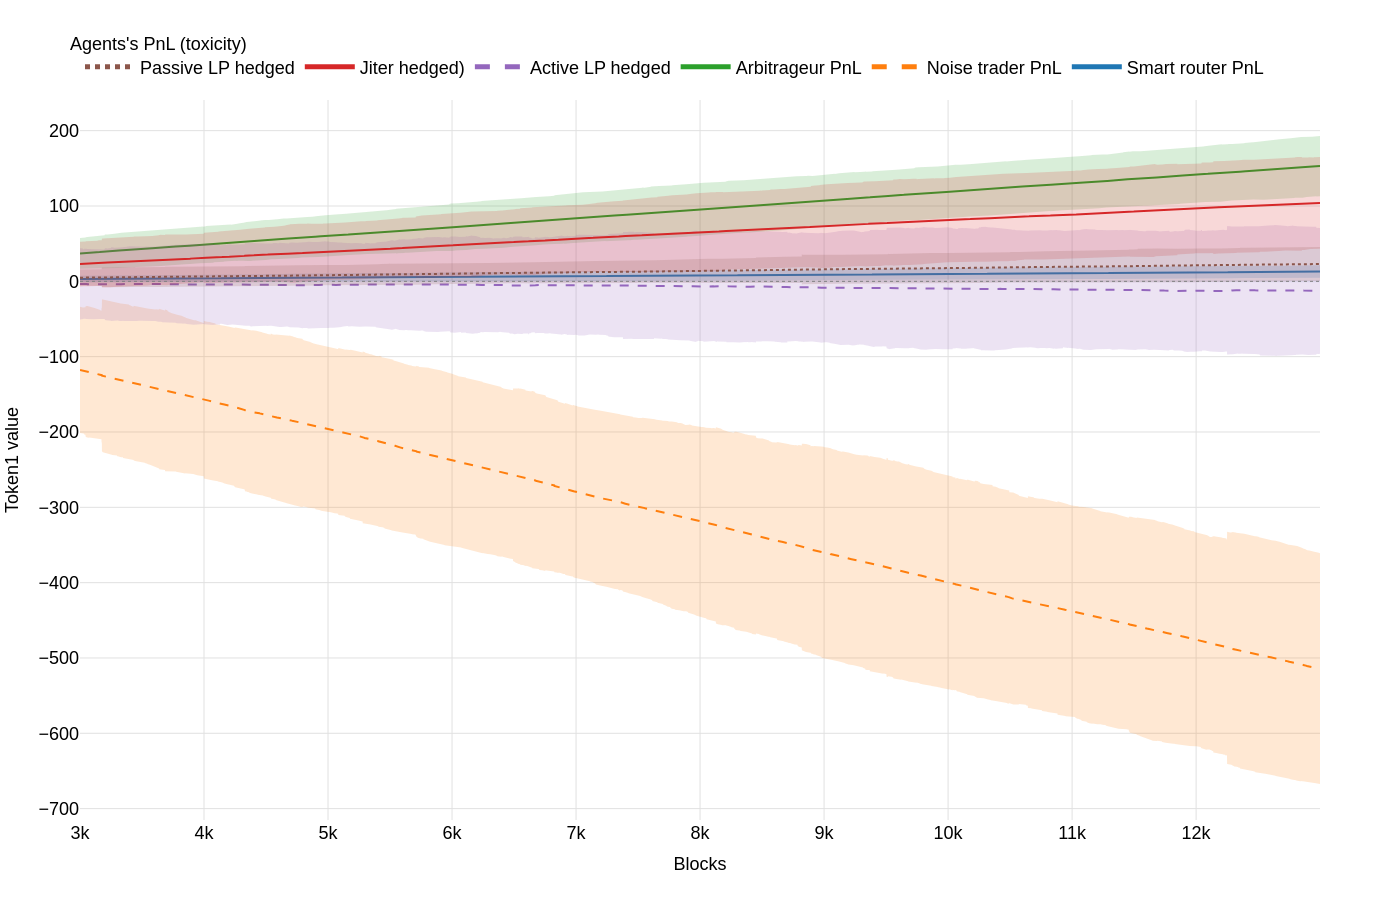
\includegraphics[width=0.8\linewidth]{images/pnl_toxicity_test_runs50_LPpassiveshare0.5_pjit1_102248.png}
    \caption{Agents' PnLs averaged across 50 runs in the toxicity fee case for model 2. The dashed area around the mean corresponds to plus/minus two standard deviations. The remaining parameters are summarized in \ref{tab:common_params}.}
    \label{fig:pnl_model2_toxicity}
\end{figure}

\begin{figure}
    \centering
    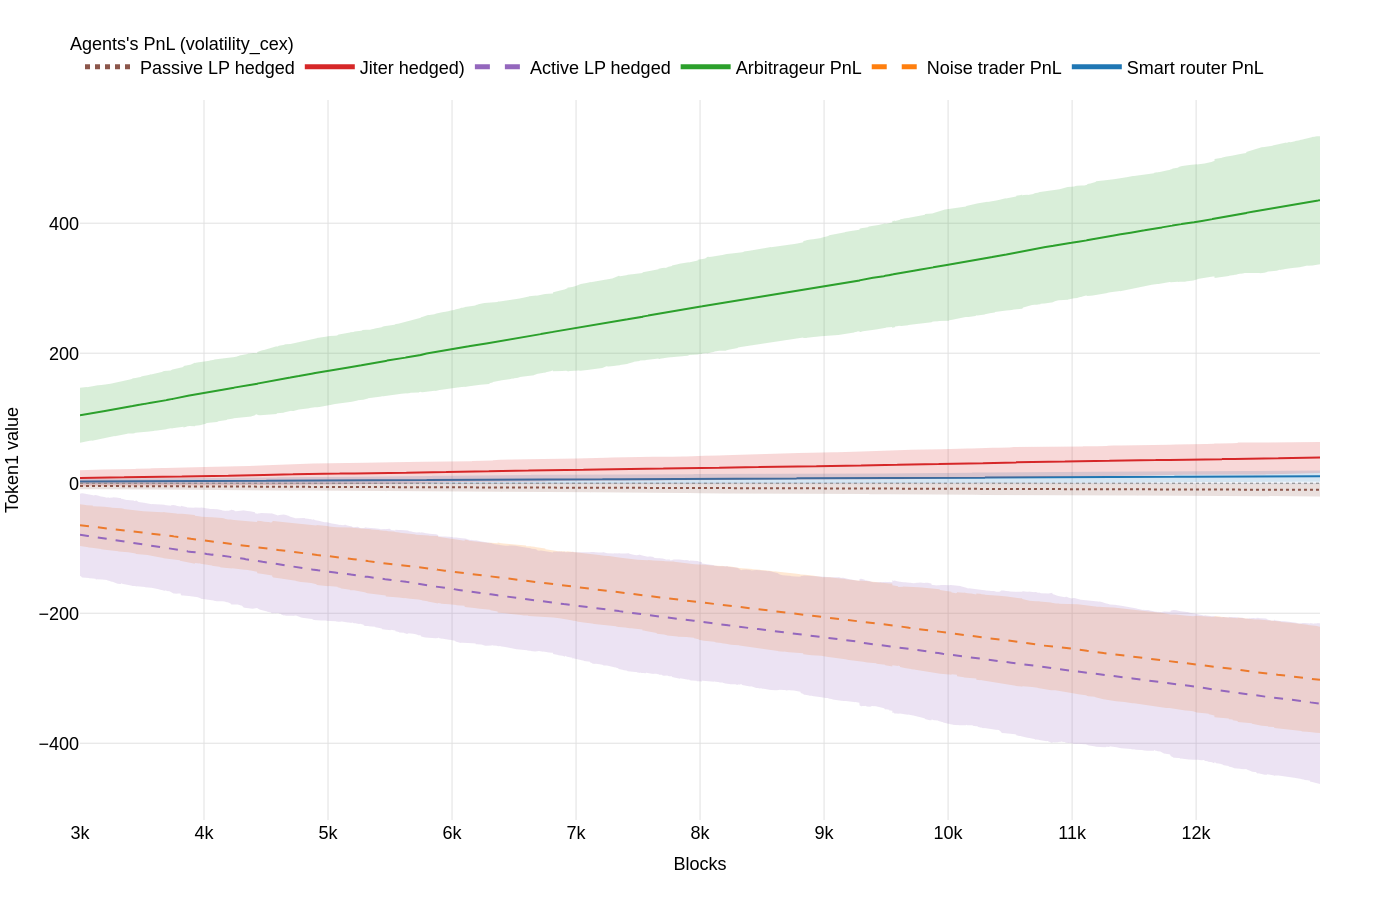
\includegraphics[width=0.8\linewidth]{images/pnl_volatility_cex_test_runs50_LPpassiveshare0.5_pjit1_141947.png}
    \caption{Agents' PnLs averaged across 50 runs in the CEX volatility-driven fee case for model 2. The dashed area around the mean corresponds to plus/minus two standard deviations. The remaining parameters are summarized in \ref{tab:common_params}.}
    \label{fig:pnl_model2_volcex}
\end{figure}

\begin{table}[htbp]
    \centering
    \caption{Arbitrage-related metrics are reported as (mean,standard deviation) across model specifications. “Arb Exec” denotes the number of executed arbitrage trades, “No Arb” the number of instances in which arbitrage was infeasible because prices lay within the no-arbitrage band, and “Arb Rej” the number of arbitrage attempts rejected by the profitability filter. These quantities remain broadly stable across models and parameterizations. All remaining simulation parameters are reported in Table~\ref{tab:common_params}.}
    \label{tab:arb_detailed}
    % Resizebox is crucial here because 13 columns is too wide for standard text width
    \resizebox{\textwidth}{!}{%
        \begin{tabular}{l cccc cccc cccc}
            \toprule
            & \multicolumn{4}{c}{\textbf{Arb Exec}} & \multicolumn{4}{c}{\textbf{No Arb}} & \multicolumn{4}{c}{\textbf{Arb Rej}} \\
            \cmidrule(lr){2-5} \cmidrule(lr){6-9} \cmidrule(lr){10-13}
            \textbf{Model} & static & vol dex & vol cex & toxicity & static & vol dex & vol cex & toxicity & static & vol dex & vol cex & toxicity \\
            \midrule
            Model 0 & 9020, 75 & 5892, 60 & 6360, 86 & 5843, 104 & 3980, 75& 7108, 59& 6640, 86& 7157, 104& 0.10, 0.30& 0.04, 0.20& 0.10,0.30& 0.06, 0.24\\
            Model 1 & 8696, 62& 6008, 65& 6360, 86& 5529, 97& 4304, 62& 6992, 65& 6640, 86& 7471, 97& 0.16, 0.36& 0.06, 0.23& 0.10, 0.30& 0.12, 0.32\\
            Model 2 & 8680, 62& 6025, 61& 6092, 74& 5518, 99& 4319, 62& 6975, 61& 6908, 73& 7482, 99& 0.08, 0.27& 0.06, 0.23& 0.04, 0.19& 0.10, 0.36\\
            \bottomrule
        \end{tabular}%
    }
\end{table}


\subsection{LVR vs fees vs block size}
In this section we discuss the behaviour of the per-block ratio

\begin{equation}
    R_t = \frac{\Delta \text{LVR}_t}{\Delta F_t} \qquad \text{where} \qquad \Delta \text{LVR}_t = \text{LVR}_t-\text{LVR}_{t-1} ,\quad \Delta F_t=F_t-F_{t-1}
\end{equation}
as the size of the block increases. It quantifies how much the fee earned by the LP offset the accumulated LVR in each block.
The LVR theory implies that holding other factors fixed, the important scaling is:
\begin{equation}
  \mathbb{E}[\mathrm{LVR} \text{ over an interval of length } \Delta t]
  \;\propto\;
  \sigma^2 \,\Delta t.
  \label{eq:lvr_time_scaling}
\end{equation}
In the simulator, increasing $B$ makes each block represent a longer interval before the end-of-block price
$m_t$ is realized and before the pool is compared against it. Larger blocks therefore produce larger typical price changes within a block (variance scales with time), which increases the magnitude of mispricing and arbitrage extraction in that block, consistent with \eqref{eq:lvr_time_scaling}. This naturally produces approximately linear growth of $\Delta\text{LVR}_t$ with $B$.
However, in general, even if $\Delta\mathrm{LVR}_t$ grows with $B$, the ratio $R_T$ will only remain stable if
fee revenue also grows proportionally.
In this ABM configuration, trader arrivals are specified as expected number of trade intents per block,
not per unit of continuous time. As a result, increasing $B$ can raise LVR per block without mechanically increasing the number of fee-generating trades per block by the same factor.

Figure \ref{fig:static_vs_toxicity_ratio} shows the results of this analysis, comparing the static fee case and the toxicity-driven fee case. The main findings are:
\begin{itemize}
  \item \textbf{Static fee mode:} both passive and active LP cohorts have $\Delta\text{LVR}_t/\Delta{F}_t>1$, increasingly so at
        larger $B$. The structural adverse selection cost dominates fixed fee revenue, producing negative hedged profitability.
        Active (more concentrated) LPs tend to have the worst coverage ratios.
  \item \textbf{Toxicity fee mode:} the ratio drops below one and becomes much more stable across $B$. This indicates the controller
        is broadly successful at matching fee revenue to adverse selection intensity, restoring positive hedged profitability for LPs.
  \item \textbf{Jiter:} in toxicity mode the Jiter has $0<\Delta\text{LVR}_t/\Delta{F}_t<1$ and typically keeps a large fraction
        of fees as hedged profit (net of flash costs). In static mode the Jiter ratio appears strongly negative, but this is best
        understood as a consequence of (i) selective timing, and (ii) strong selection bias from conditioning on a tiny number of
        successful JIT executions: only a handful of extremely profitable JIT opportunities appear in the sample, pushing measured
        $\Delta\text{LVR}_t$ negative.
\end{itemize}

\begin{figure}[h]
  \centering

  \begin{subfigure}{\linewidth}
    \centering
    \caption*{\textbf{Static}}
    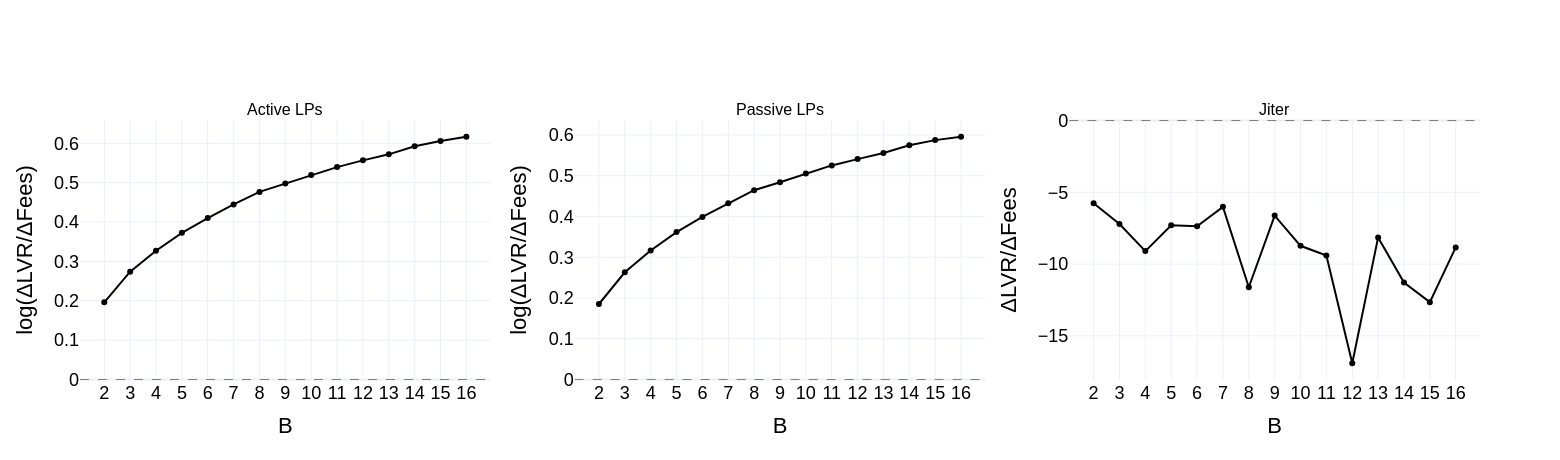
\includegraphics[width=\linewidth]{images/dLVR_over_dFees_medians_vs_block_time_static_flow_test_runs50_pid42657.png}
  \end{subfigure}

  \vspace{0.5em}

  \begin{subfigure}{\linewidth}
    \centering
    \caption*{\textbf{Toxicity}}
    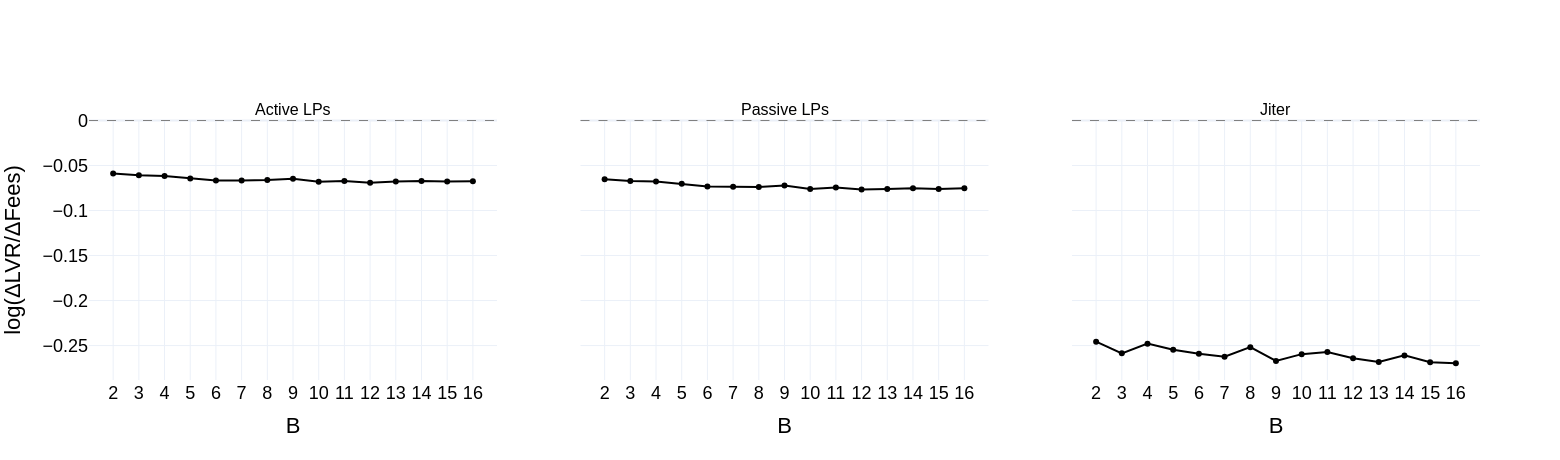
\includegraphics[width=\linewidth]{images/dLVR_over_dFees_medians_vs_block_time_toxicity_flow_test_runs50_pid14207.png}
  \end{subfigure}

  \caption{Median of $r=\Delta\mathrm{LVR}/\Delta\mathrm{Fees}$ vs block time $B$ for active+passive LPs and Jiter.}
  \label{fig:static_vs_toxicity_ratio}
\end{figure}


\section{Conclusions}

This paper introduced a granular agent-based laboratory for studying the economics of Uniswap v3 liquidity provision under realistic blockchain frictions and heterogeneous strategic behavior. The model couples a concentrated-liquidity AMM to a reference CEX whose mid-price follows a stochastic-volatility Heston dynamics with permanent impact induced by trades, and embeds a block-based settlement layer with mempool latency and stochastic transaction ordering. Within this environment, arbitrageurs enforce a no-arbitrage band shaped by taker fees and flash-loan costs, while liquidity takers split across an uninformed noise-trader component and a best-execution smart router that endogenizes the DEX share as fees and liquidity conditions change. Liquidity providers are modeled as cash-budgeted agents who mint/burn positions with heterogeneous review clocks, range-selection rules, and risk-management triggers. The framework implements a discrete-time rebalancing benchmark that preserves self-financing and inventory matching, enabling a clean decomposition of outcomes into fees versus Loss-Versus-Rebalancing (LVR) and thus a direct measurement of “hedged PnL” as the economically relevant profitability metric for liquidity provision. 

Across the baseline configurations, the simulations confirm a central microstructure mechanism: in a block-based system, transient within-block deviations between DEX and CEX prices generate systematic arbitrage opportunities that translate into LVR, especially when liquidity is concentrated near the current price and the AMM effectively posts stale quotes. In Model 0, a static fee produces persistently negative hedged PnL for passive LPs, despite a non-trivial fraction of flow routed to the DEX by the smart router. Allowing the taker fee to adapt according to an underlying signal changes the balance between fee income and adverse selection. Among the tested controllers, the toxicity-based schedule, constructed from an excess-basis proxy measuring how much the DEX price gap exceeds the contemporaneous fee band, post effectively internalizes arbitrage intensity: it raises fees specifically in regimes where stale-price risk is highest, leading to positive hedged PnL for passive LPs while maintaining a stable (though reduced) DEX market share. Volatility-based schedules also improve LP outcomes relative to the static benchmark, but generally deliver weaker gains, consistent with volatility being a noisier and less targeted proxy for the realized adverse selection channel driving LVR in this microstructure.

Model 1 highlights a core trade-off created by concentrated liquidity. Introducing active LPs increases depth near the prevailing price, improving DEX competitiveness and raising the router’s DEX share; however, the same concentration amplifies exposure to LVR, pushing active LP hedged PnL below that of passive LPs under most fee regimes. Notably, the toxicity-driven controller is the only specification in which both passive and active LP cohorts achieve positive hedged profits, underscoring that where and when fees respond matters more than simply charging higher fees on average. In other words, adaptive pricing can be beneficial, but only if the control signal is aligned with the microstructural source of adverse selection rather than with broad market variability alone.

Model 2 introduces an MEV searcher performing Just-In-Time (JIT) liquidity. The results emphasize a second, protocol-design-relevant tension: mechanisms that protect LPs from arbitrage (dynamic fees) can simultaneously increase the returns to latency/priority strategies that appropriate fee flow. In the static-fee setting, the JIT agent is approximately break-even, whiYou have to highlight what is the problem at handle other LP cohorts remain negative on a hedged basis. Under dynamic fees, the JIT strategy becomes profitable, because it can time liquidity to capture elevated fees while keeping inventory exposure short-lived, yet passive and active LPs fail to attain positive hedged PnL under any of the tested schedules. This outcome is economically coherent: when large swaps are systematically wrapped by JIT liquidity, the fee stream that would otherwise compensate longer-horizon LPs is diverted to the searcher precisely during the most lucrative blocks, leaving residual LPs to bear LVR without sufficient fee income.

Overall, the experiments support three broad conclusions. First, LVR is fundamentally a microstructure cost, magnified by discrete-time execution and latency, and it is better evaluated through modeling the execution layer and not just via continuous-time diffusion intuition. Second, dynamic fees can improve the sustainability of liquidity provision, but effectiveness depends on using signals that are tightly linked to adverse selection (e.g., excess basis/toxicity) and on managing the endogenous response of order routing. Third, MEV/JIT dynamics can dominate the distribution of fee revenue, potentially negating the benefits of adaptive fees for ordinary LPs unless fee mechanisms and execution rules are co-designed with MEV-resilience in mind.

These findings suggest several directions for future work within the same ABM framework: (i) calibrating agent intensities and parameter regimes to specific pools and chains to connect qualitative insights to empirical magnitudes; (ii) incorporating explicit gas costs, priority fees, and auction-style ordering to model the full MEV supply chain; (iii) extending fee controllers to include anti-JIT features (e.g., time-weighted fee attribution, liquidity “stickiness” requirements, or penalties for ultra-short-lived liquidity) while quantifying welfare impacts on takers and routers; and (iv) studying multi-pool routing and cross-pool arbitrage, where dynamic fees in one venue propagate strategically to others. Taken together, the ABM developed here provides a controlled, interpretable testbed showing that adaptive pricing is a promising—but not standalone—tool for improving LP economics in concentrated-liquidity AMMs operating under realistic blockchain microstructure. 


\bibliographystyle{abbrv}
\bibliography{bibliography}
% \section*{References}

% \begin{enumerate}[label={[\arabic*]}]
%   \item G. Angeris, A. Chitra, A. Alexandrov, and T. Roughgarden,
%         ``An Analysis of Uniswap Markets,'' 2020.
%   \item P. Milionis, C. Moallemi, and T. Roughgarden,
%         ``Automated Market Making and Loss Versus Rebalancing,'' 2023.
% \end{enumerate}

% \appendix
% \section{Appendix}
% \subsection{Discrete-Time Implementation of Heston dynamics}
% In the simulation, the continuous system is discretized using an Euler-Maruyama scheme with full truncation to ensure the non-negativity of the variance process. For a time step size $\Delta t$ (corresponding to one micro-step), we draw two independent standard normal variables $Z_1, Z_2 \sim \mathcal{N}(0,1)$.

% First, the variance update step is computed. To prevent numerical instability where $v_t$ might become negative, we apply a truncation scheme:
% \begin{equation}
%     \tilde{v}_{t} = \max(v_t, 0).
% \end{equation}
% The increment is calculated as:
% \begin{equation}
%     \Delta v_t = \kappa(\theta - v_t)\Delta t + \sigma_v \sqrt{\tilde{v}_{t}}\sqrt{\Delta t} Z_1.
% \end{equation}
% The variance for the next step is then fully truncated:
% \begin{equation}
%     v_{t+\Delta t} = \max(0, v_t + \Delta v_t).
% \end{equation}

% Second, the log-price is updated using a correlated shock $Z_{price}$:
% \begin{equation}
%     Z_{price} = \rho Z_1 + \sqrt{1 - \rho^2} Z_2.
% \end{equation}
% The log-price update follows:
% \begin{equation}
%     \ln m_{t+\Delta t} = \ln m_t + \left(\mu - \frac{1}{2}\tilde{v}_{t}\right)\Delta t + \sqrt{\tilde{v}_{t}}\sqrt{\Delta t} Z_{price}.
% \end{equation}

% This formulation allows the reference market to exhibit rich dynamics where the instantaneous volatility $\sigma_t = \sqrt{v_t}$ fluctuates stochastically, providing a more rigorous test environment for liquidity provision strategies than static GBM baselines.

\end{document}
